\chapter{Implementation of short-range machine learning interatomic potentials}
%\section{Modular design of MLIP}

Interatomic potentials have been used since long time to approximate the potential energy surface in classical molecular dynamics (MD) simulation by decomposing the systems' total energy into body-order contributions.
This is done by solving the classicals equations of motions of the system of interest
%In the picture of the Born-Oppenheimer approximation we can decouple the time propagation of the nuceil and electronic.the potential energy quantum mechanically
\begin{subequations}
\begin{align}
  H(\mathbf{p}, \mathbf{q}) = \frac{\mathbf{p}^2}{2m} + V(\mathbf{q}),\quad
  \frac{\partial\mathbf{p}}{\partial t} = \frac{\partial V(\mathbf{q})}{\partial\mathbf{q}},\quad\frac{\partial\mathbf{q}}{\partial t} = \frac{\mathbf{p}}{m}\quad\textrm{(classical Hamiltonian mechanics)},
\end{align}\\
\end{subequations}
with an interatomic potential of the form
\begin{subequations}
\begin{gather}
  V(\mathbf{q}) = \sum_{i = 1} V_1(\mathbf{r}_i) + \sum_{i,j = 1} V_2(\mathbf{r}_i, \mathbf{r}_j) + \sum_{i,j,k = 1} V_3(\mathbf{r}_i, \mathbf{r}_j, \mathbf{r}_k) + \ldots \quad\textrm{(interatomic potential)}.
\end{gather}
\end{subequations}
Due to the limitation in the computational power, the development of accurate interatomic potentials historically relied on a meticulous hand-tuning of parametric models called \emph{empirical interatomic potential}.
They were constrained by the chemical and phase space they could predict accurately~\cite{stillinger1985computer, tersoff1988empirical}.
However, with the increased computational power available today, the shift towards data-driven models emerged allowing a more automatized construction for fitting models on data generated from empirical potentials~\cite{blank1995neural} or ab initio calculations~\cite{brown2003classical,lorenz2006descriptions,behl-parr07prl}.
Remarkably, the current generation of machine learning interatomic potentials (MLIP) have reached the capability to extensively cover chemical~\cite{lopanitsyna2023modeling} and phase space~\cite{bartok2018machine} accurately.

The abundance of ML packages available today~\cite{Haddad2023Artificial}, such as \texttt{scikit-learn}~\cite{pedregosa2011scikit}, \texttt{PyTorch}~\cite{NEURIPS2019_9015}, prompts the question of whether we need to develop a new ML package.
%the need for a new ML package for the development of MLIPs.
Most of these packages, however, are focused on applications in generic data analysis and computer vision, and are therefore not suited to the specific needs of MLIPs, which include domain-specific featurization of 3D structures and gradient inference as the calculation of forces requires. % with respect to target properties.
To ensure that the code base remains manageable, strategic integration with existing software solutions is essential, wherever appropriate.
%To keep development and maintenance efforts of the code base manageable it is necessary to integrate with existing software solutions where adequate.
This requires not only a solid understanding of relevant mathematical methods but also proficiency in current software tools.
This combination of requirements poses a significant challenge in the development of enduring and robust MLIP packages.
%To reduce the development and maintainance costs it is necessary to find points in ones method where already established software packages can be embedded in.
%For that a mathematical and algorithmic understanding of the landscape of methods and proficient skills in software development are needed which makes it such challenging problem.
 % tlerefore cannot be directly embedded for the development of MLIP.
%symmetrization of features based on point clouds in 3D
%symmetrized features in three-dimensional space 
%  are not requirements that are shared with many other domains that deploy ML models.
%This has be considered from multiple aspects does an interface happen without much loose in performance cost, is the maintainance cost of the interface lower than creating a implemantion.
%software development of MLIP remains challenging problem as most of the packages in the
%which is not a requirement that is not much shared with other domains.
%Secondly, the 
%the ML models rely on a featurization of data which is domain-dependent and therefore requires the development custom software.
%the creation of a model the shipping to an MD software.
%While featurization is domain-specific and needs custom implementations also the existing ML software ecosystem can often not to be reused for our domain as including gradients into the pictures completely changes the constraints on the required software.
%The gradient computation shifts the bottleneck drastically and thus changes the existing algorithmic design.

In this chapter, I discuss my contributions to the software ecosystem that facilitates the deployment of MLIPs into an MD software.
These contributions include my work to the \texttt{librascal} package~\cite{LIBRASCAL}, instrumental for constructing MLIPs based on the SOAP featurization of atomic structures and the \texttt{scikit-matter}~\cite{goscinski2023scikit} package -- a toolkit for various data-driven preprocessing methods that facilitate the MLIP construction. % as feature and sample selection.
Additionally, I implemented an interface to \texttt{LAMMPS}~\cite{LAMMPS}, a state of the art classical MD code, enabling the studies on ferroelectric phase transitions in barium titanate, as detailed in Ref.~\cite{gigli2023modeling} and on the transport properties of lithium ortho-thiophosphate, as described in Ref.~\cite{gigli2023mechanism}.
Finally, we briefly discuss how the package \texttt{metatensor}~\cite{metatensor} enable a more modular approach to build MLIPs.

\section{Implementation of cubic splines for featurization}
\label{sec:cubic_spline}
%As part my work in the first year, I participated in the development of a library designed to allow efficient computation of atomic density based descriptors, named librascal.
%The library is designed with most emphasize on efficiency with regard to code structure and computation methods of descriptors.
%The code structure is focused on reducing runtime cost by allowing a contiguous iteration through atomic environments and by applying template based methods as curiously recurring template pattern (CRTP) to prevent runtime lookups of virtual functions with the tradeoff of higher compile time costs.
One of main contributions to \texttt{librascal} has been the implementation of a cubic spline to interpolate the radial expansion coefficients as expressed in Eq.~\eqref{eq:radial_expansion}.
%iin the last year has been the development of efficient methods for the computation of the radial basis expansion for the SOAP descriptor.
%In contrast to the approaches discussed in Section~\ref{sec:evaluation_of_radial_contribution}, for librascal Gaussian typed orbital (GTO) functions are used as radial basis functions 
%\begin{subequations}
%\begin{align}
%R_n^{GTO}(r) = r^{n+2}\exp(-b_nr^2)N_n,\hspace{5em}\\
%\text{with } b_n = 1/(2\sigma_n),\quad \sigma_n = r_c\,\textrm{max}(\sqrt{n},1)/n_{\text{max}},
%% Remark: I added the factor r^2 to the basis function to be comparable with other publications
%\end{align}
%\end{subequations}
%Performance test done with the descriptor library Dscribe show a speed up of $10.07\pm 0.56$ times of the GTO basis over the polynomial one\cite{himanen2020dscribe}.
%In librascal the GTO improve the expansion on the radial part is to separate the radial and angular part in the original atomic density function as proposed by Marco...
%that allowed further works
%the computation analytically the integral for the radial expansion in Eq.~\eqref{eq:radial_part_in_spherical_expansion}. 
%However, due to the modified spherical Bessel function $i_l$ %in Eq.~\eqref{eq:radial_part_in_spherical_expansion}
%an analytical expansion of radial term requires the evaluation of the computationally expensive confluent hypergeometric function $\hyponefone$ 
%\begin{multline}
%    \label{eq:radial_integral}
%    \int_0^{\infty} R_n^{GTO}(r) \exp[-a(r^2+r_{ij}^2)]i_l(2arr_{ij}) \,\mathrm{d}r
%    %\langle rlm|\mathcal{X}_i\rangle_{\hat{R}\hat{t}}\,\mathrm{d}r
%    = N_n \pi^{\frac32}\frac{\Gamma(\frac{n+l+3}{2})}{\Gamma(l+\frac32)} \\
%    (a+b)^{-\frac{n+l+3}{2}} (ar_{ij})^l \exp[-ar_{ij}^2] \hyponefone\big(\frac{n+l+3}{2},l+\frac32,\frac{a^2r_{ij}^2}{a+b}\big) = f^{nl}(r_{ij}).
%\end{multline}
%The contribution of this function to the overall cost of the radial expansion can be seen in Fig.~\ref{fig:hyp1f1_contribution} ranging from 55\% to 75\%  of the total time.F
For each coefficient $nl$, the one-dimensional function $f^{nl}:[0,r_c]\rightarrow\mathbb{R}$ is splined.
The function $f^{nl}$ maps the distance $r\in[0,r_c]$ to the neighbor contribution of the radial expansion coefficient as in Eq.~\eqref{eq:radial_expansion}.
For the construction of the cubic spline the targeted interval $[0,r_c]$ is further partitioned into a set of subintervals $[r_1, r_2], \ldots, [r_{K}, r_{K+1}]$ where $0 = r_1 < r_2 < \ldots < r_{K} < r_{K+1} = r_c$.
Then cubic splines are order 3 polynomials $p_k(r) = A_k + B_kr + C_kr^2 + D_kr^3$ on the interval $[0,1]$ with the boundary conditions
%The radial expansion coefficients are evaluated for each of the distances $r_1 < r_2 < \ldots < r_{K+1}$ to set up a set of conditions
%The end points of each subinterval are evaluated with the origin approximated by a cubic polynomial boundary conditions.
%Let $\{r_k\}_{k=1}^{M+1}$ be the set of $M+1$ boundary points in the interval $[0,r_c]$, then cubic spline defines polynomials $p_k(r) = A_k + B_kr + C_kr^2 + D_kr^3$ on the interval $[0,1]$ with the boundary conditions
\begin{subequations}
\label{eq:abscissas_boundary_conditions}
\begin{gather}
    p^{nl}_{k}(0) = f^{nl}(r_k)\text{ and } p^{nl}_{k}(1) =  f^{nl}(r_{k+1})\text{ for } k=1,\ldots,K , \label{eq:function_boundary_conditions}\\
    %p^{nl}_{k}(0) = p^{nl}_{k-1}(1)&\text{ and }
    \left(\frac{\partial p^{nl}_{k}}{\partial r}\right)_{r=1} = \left(\frac{\partial p^{nl}_{k+1}}{\partial r}\right)_{r=0} \text{ for } k=1,\ldots,K-1  ,\label{eq:derivative_boundary_conditions}\\
    \left(\frac{\partial^2 p^{nl}_{k}}{\partial r^2}\right)_{r=1} = \left(\frac{\partial^2 p^{nl}_{k+1}}{\partial^2 r}\right)_{r=0} \text{ for } k=1,\ldots,K-1  ,\label{eq:second_derivative_boundary_conditions}\\
    %p^{nl}_k(1) = p^{nl}_{k+1}(0)&\text{ and }  \left(\frac{\partial p^{nl}_k}{\partial r}\right)_{r=1} = \left(\frac{\partial p^{nl}_{k+1}}{\partial r}\right)_{r=0} \text{ for } k=1,\ldots,K-1 ,\label{eq:derivative_boundary_conditions}\\
    \left(\frac{\partial^2 p^{nl}_{1}}{\partial r^2}\right)_{r=0} = 0\text{ and } \left(\frac{\partial^2 p^{nl}_{K}}{\partial r^2}\right)_{r=1}=0\quad\text{(natural boundary conditions)}.\label{eq:natural_boundary_conditions}
\end{gather}
\end{subequations}
%The boundary conditions ensure the continuity.
These $4K$ boundary conditions can be rearranged to a tridiagonal linear system solving for the $4K$ unknowns~\cite{bartels1998hermite}
%\begin{subequations}
%\begin{align}
%  \left(\frac{\partial p^{nl}_{k}}{\partial r}\right)_{r=0} &= B_k \\
%  \left(\frac{\partial p^{nl}_{k}}{\partial r}\right)_{r=1} &= B_{k+1} = B_k + 2C_k + 3D_k \\
%  \left(\frac{\partial^2 p^{nl}_{1}}{\partial r^2}\right)_{r=0} &= 0 = 2C_1 \\
%  \left(\frac{\partial^2 p^{nl}_{K}}{\partial r^2}\right)_{r=1} &= 0 = 2C_{K} + 6D_K \Rightarrow C_K = - 3D_K
%  p^{nl}(0) &= A_k \\
%  p^{nl}(1) &= A_{k+1} = A_k + B_k + C_k + D_k \\
%  \Rightarrow p^{nl}(1)-p^{nl}(0) &= B_k + C_k + D_k\\
%  \Rightarrow 3(p^{nl}(1)-p^{nl}(0)) &= 3B_k + 3C_k + 3D_k \\
%\end{align}
%\end{subequations}
%\begin{subequations}
%\begin{align}
%   0 = 2C_{k} + 3D_k
%  p^{nl}(1) - p^{nl}(0) k =
%  p^{nl}(0) &= A_k \\
%  p^{nl}(1) &= A_{k+1} = A_k + B_k + C_k + D_k \\
%  \left(\frac{\partial p^{nl}_{k}}{\partial r}\right)_{r=0} &= B_k \\
%  \left(\frac{\partial p^{nl}_{k}}{\partial r}\right)_{r=1} &= B_{k+1} = B_k + 2C_k + 3D_k
%\end{align}
%\end{subequations}
\begin{subequations}
\begin{align}
%A_k = f^{nl}(r_k),\quad C_k = 3(f^{nl}(r_{k+1})-f^{nl}(r_k)) - 2B_k-B_{k+1},\\
%D_k = 2(f^{nl}(r_{k})-f^{nl}(r_{k+1})) + B_k+B_{k+1},\hspace{5em}\\
\begin{pmatrix}
    2 & 1       &           &       &    \\
    1 & 4       & 1         &           &    \\
      & \ddots  & \ddots    & \ddots    &           \\
      &         & 1         &     4     & 1   \\
      &         &           &     1     & 2
\end{pmatrix}
\begin{pmatrix}
B_1\\
B_2\\
\vdots\\
B_{K-1}\\
B_{K}
\end{pmatrix}
=
\begin{pmatrix}
3(f^{nl}(r_2)-f^{nl}(r_1))\\
3(f^{nl}(r_3)-f^{nl}(r_1))\\
\vdots\\
3(f^{nl}(r_K)-f^{nl}(r_{K-2}))\\
3(f^{nl}(r_K)-f^{nl}(r_{K-1}))
\end{pmatrix}.
\end{align}
\end{subequations}
This system can be solved in linear time with time complexity $O(2K)$ by iterating two times through the matrix following a Gaussian elimination scheme.
%\begin{equation}
%    
%\end{equation}
%In the forward pass the lower off diagonal is eliminated to zero, in the backward path the upper path is eliminated to zero.
%Commonly, for interpolators the grid size is adaptively changed until it is below an error bound given by the user as input.
The grid points $\{r_k\}_{k=0}^{K+1}$ are incrementally adjusted until the function approximation error falls beneath a user-specified error threshold.
The approximation error can be estimated by sampling points in the intervals $(r_k, r_{k+1})$ and computing the difference between the function $f^{nl}$ and the spline $p^{nl}$.
During implementation, it has been found that conditioning on both, the relative and absolute error, yields the most robust results in terms of interpolation accuracy and convergence of the grid size.
While algorithms for adaptive grids can be advantageous to control the grid size and thus reduce memory requirements, it has been found that using a uniform grid does not reach a memory intensive regime while having minimal impact on the prediction accuracy.
This is evidenced by experiments on chemical shieldings of hydrogen environments~\cite{paruzzo2018chemical} presented in Fig.~\ref{fig:chemical_shift-spline}.
%as it can be seen in Fig.~\ref{TODO} with experiments on the chemical shieldings\cite{TOOD}.
%A point $r$ can be evaluated by first determining the corresponding boundary point $r_k$ for which $r\in[r_k,r_{k+1}]$, and then mapping $[r_k,r_{k+1}]$ to the polynomial interval $[0,1]$ with $p_k((r-r_k)/(r_{k+1}-r_k))$.
%For an arbitrary grid with $K+1$ points, the optimal complexity for searching the boundary point $r_k$ is $O(\log(M+1))$ with a binary searchc.
%\begin{equation}
%    k = \min(K,\lfloor (r-r_1)\Delta \rfloor+1), \quad \Delta = (K+1)/(r_{K+1}-r_1).
%\end{equation}
Compared to an adaptive grid the uniform grid reduces the asymptotic complexity of determining the subinterval for evaluation from a logarithmic $O(\log K)$ binary tree search to a constant $O(1)$ lookup.
Moreover, as the grid is constructed for each $nl$ channel, the setup and the evaluation of the spline opens the possibility to parallelize the spline evaluation over all channels.
Viable forms of parallelization encompass multithreading, the use of single instruction multiple data (SIMD) instructions, or leveraging graphics processing unit (GPU) acceleration.
%On the other hand for uniform grids the search time can be reduced to $O(1)$ by
%A non-uniform grid can keep the size of the grid to a minimum by only adding boundary points corresponding to the intervals with the highest error.
%This minimizes the number of evaluations of the costly function $f^{nl}$.
%With increasing number of evaluations of the function $f^{nl}$ the uniform grid will be always the better choice.
%Even though for realistic datasets with a limited number of evaluations this overhead could be crucial, it has been shown during implementation that the space overhead of a uniform grid is insignificant in comparison to the higher time complexity of the non-uniform grid.
%\begin{figure}
%    \centering
%    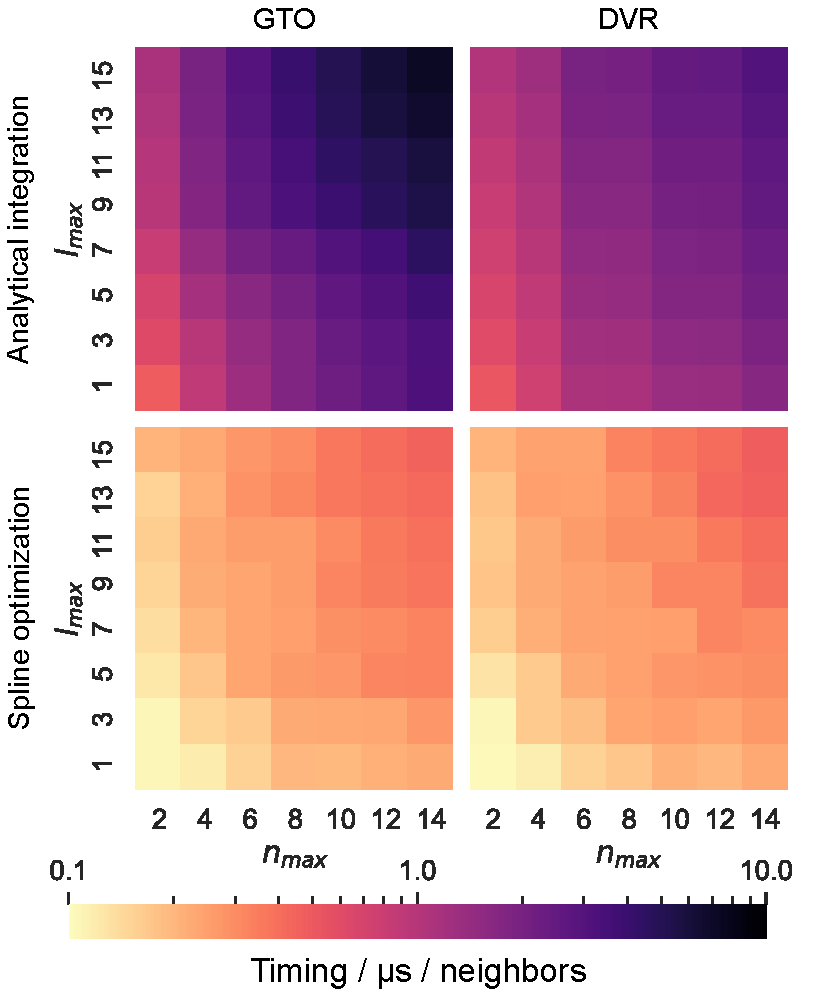
\includegraphics[width=0.5\textwidth]{fig/radial-basis.pdf}
%    \caption{Computational cost for the evaluation of the radial integral and its derivatives with different methods, for structures taken from the QM9 dataset. Note that the dataset has very little influence on this benchmark since the radial integral and its derivative are always evaluated once per neighbor. For the splining an accuracy of $10^{-8}$ was chosen}
%    \label{fig:radial-basis}
%\end{figure}

\begin{figure}
    \centering
    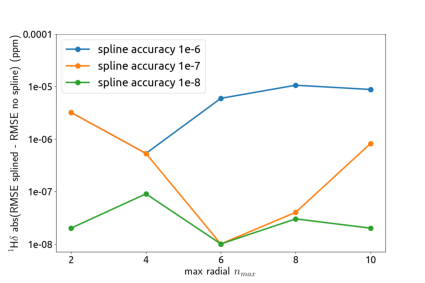
\includegraphics[width=0.7\textwidth]{fig/spline-accuracy-v2.pdf}
    \caption{The relationship of the spline accuracy on the prediction difference for chemical shieldings of hydrogen environments as conducted in Ref.~\cite{paruzzo2018chemical} for a linear model using SOAP descriptors with $l_\textrm{max}=9$.
    The impact of the spline accuracy on the difference in prediction of the chemical shifts is several magnitudes below the DFT accuracy, which is estimated to be on the order of $10^{-1}$.}
    \label{fig:chemical_shift-spline}
\end{figure}
%\begin{figure}
%    \centering
%    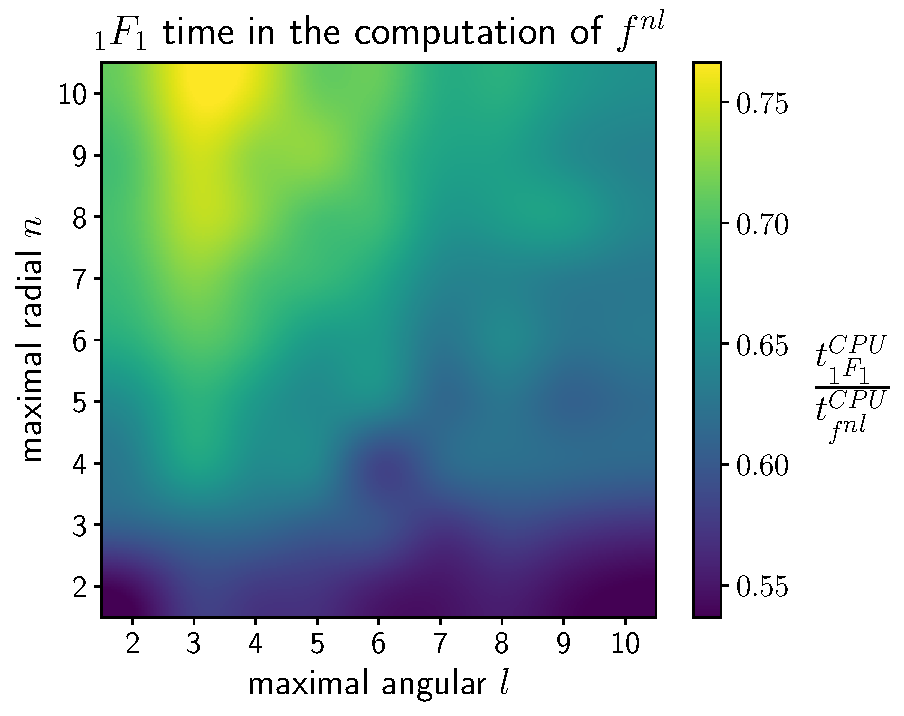
\includegraphics[width=0.5\textwidth]{fig/fig_hyp1f1_contribution_in_radial_contribution.pdf}
%    \caption{}
%    \label{fig:hyp1f1_contribution}
%\end{figure}
%\begin{figure}
%    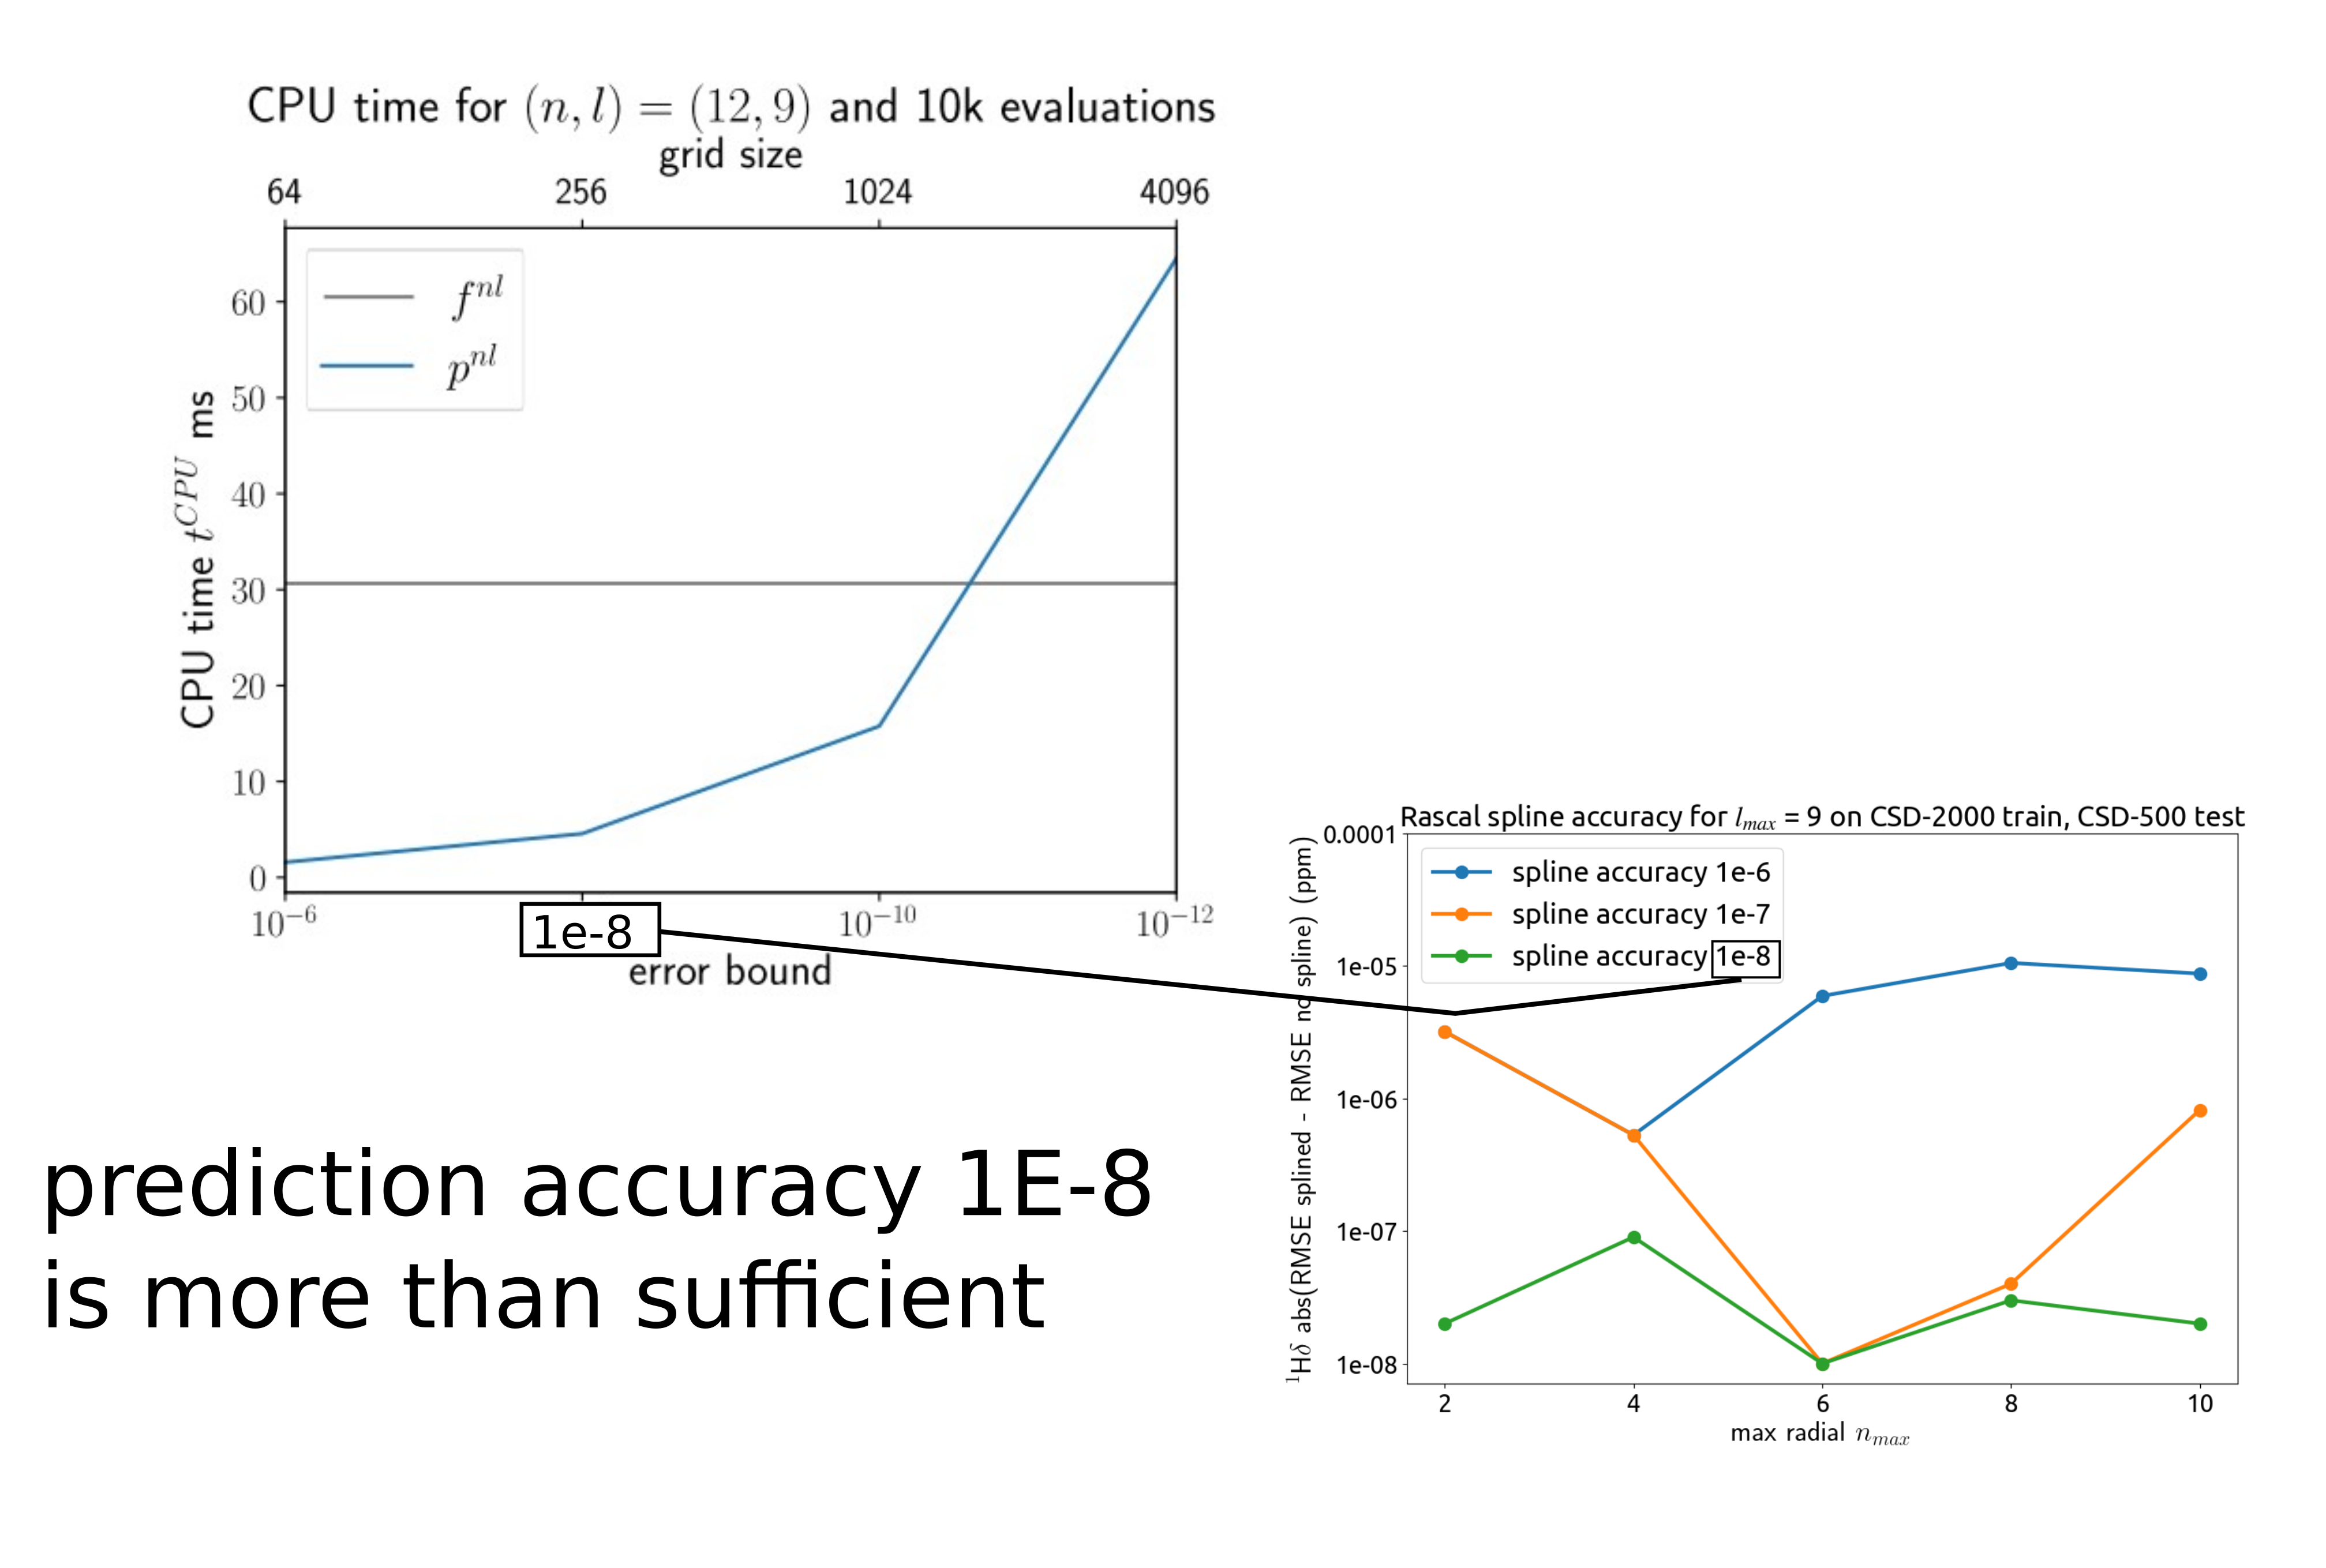
\includegraphics[width=\textwidth]{fig/slide20_2.png}
%    \caption{Effect of accuracy on prediction error}
%    \label{fig:spline-accuracy-prediction-error}
%\end{figure}\\
%\begin{figure}
%    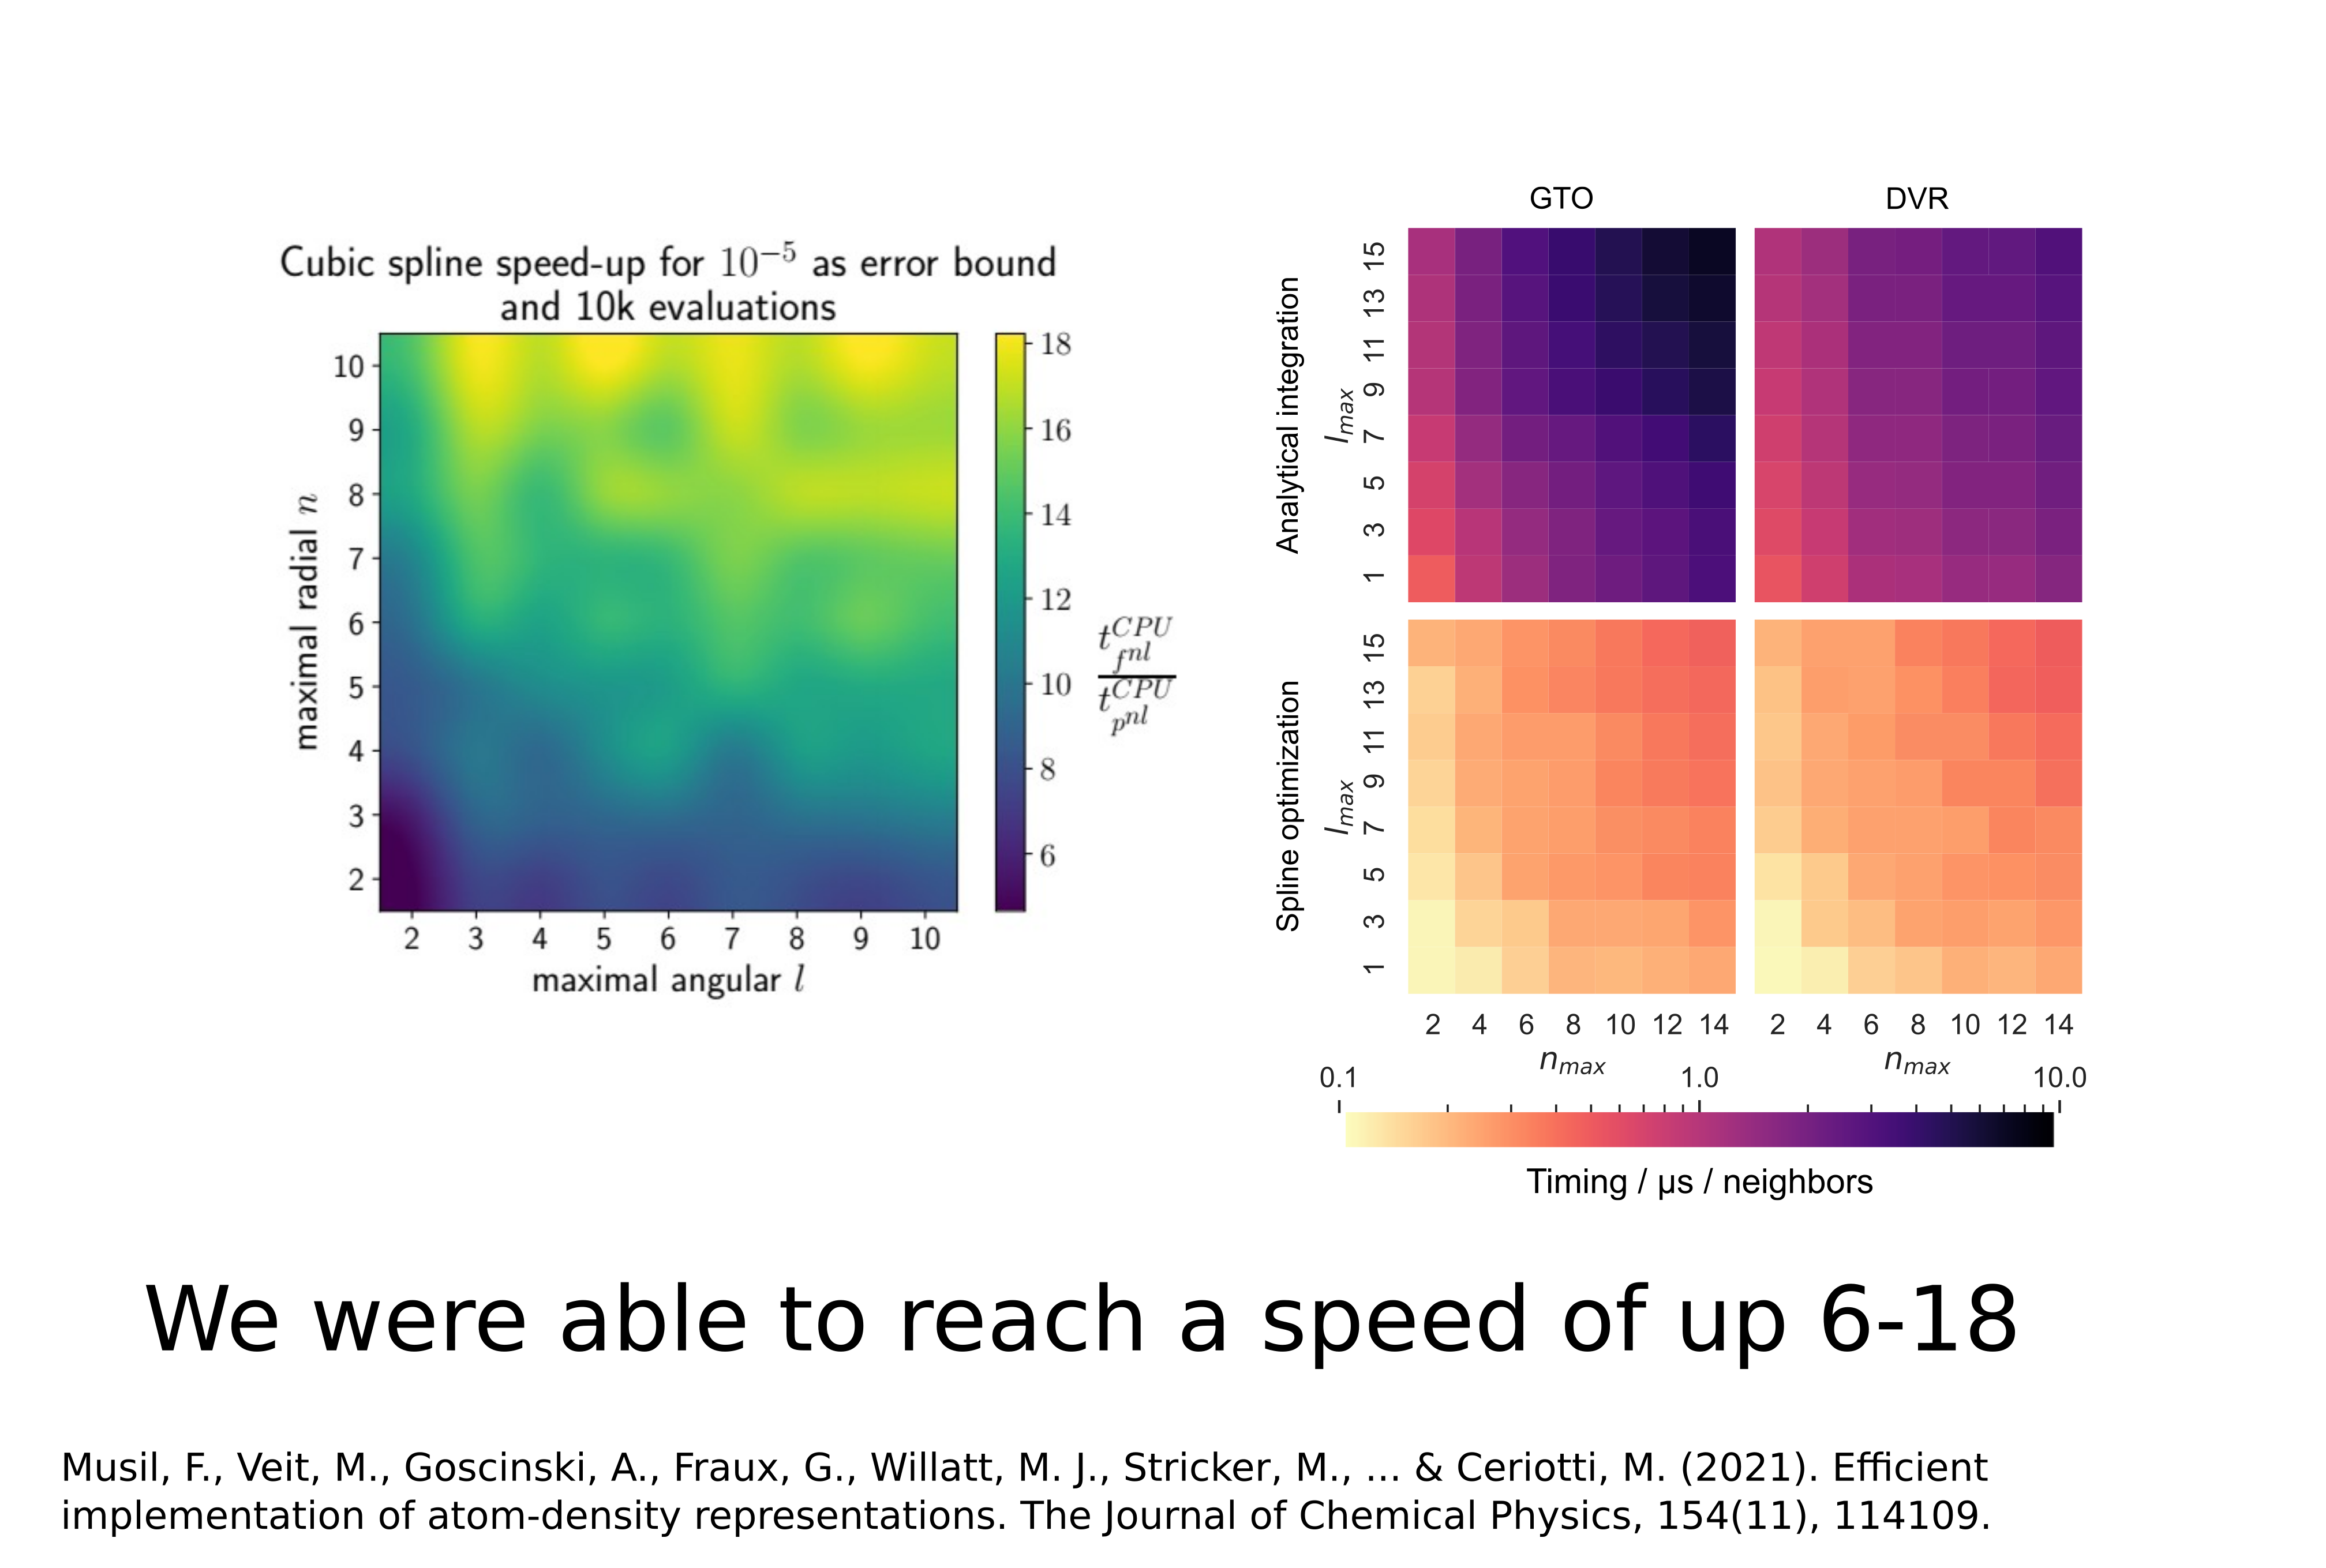
\includegraphics[width=\textwidth]{fig/slide20_3.png}
%    \caption{Speedups}
%    \label{fig:spline-speedups}
%\end{figure}

\section{Interfacing with molecular dynamics packages}
%To make such simulations possible I implemented an interface with \texttt{LAMMPS} for our in-lab developed machine learning package \texttt{librascal} to exploit the implemented domain decomposition in \texttt{LAMMPS}.
%The correction of implementation was verified by comparing the trajectories with the MLIP package \texttt{QUIP}.
%The correctness of the interwork with LAMMPS domain decomposition was verified by running a simulation for different MPI tasks and comparing the results.
%This allowed obtain results...
Molecular dynamics (MD) packages, such as LAMMPS, GROMACS, CP2K, and i-PI~\cite{LAMMPS,hess+08jctc,kuhne2020cp2k,kapil2019pi}, commonly separate the time evolution into separate modules: The time integrator to propagate equation of motions, the thermo- and barostats and the calculation and the potential energy and its forces.
%Molecular dynamics (MD) packages, such as LAMMPS, GROMACS, CP2K, and i-PI~\cite{LAMMPS,hess+08jctc,kuhne2020cp2k,kapil2019pi}, commonly isolate the computation of the potential energy into a single module disentangled from the construction of the neighbor list TODO(neihgbor list defined the thesis).
As the computation of the potential energy only depends the atomic positions and species, and the dynamics require only the energy and forces, is therefore a well-suited point for separating it from the rest of the code base.
One significant benefit of this approach is to avoid reimplementing established time integrators, thermo- and barostats.
Although their implementation may appear straightforward, developing a robust code base that transparently handles edge cases for the non-expert user is nevertheless time-consuming task, demanding extensive documentation.
Furthermore, well-established MD software packages, such as \texttt{GROMACS}~\cite{abraham2015gromacs} and \texttt{LAMMPS}~\cite{LAMMPS}, offer a variety of parallelization strategies that significantly improve the speed of interatomic potentials.
These include a message-passing interface (MPI) for the domain decomposition, CUDA- and OpenMP-based multithreading as well as SIMD abstraction modules for hardware-adaptive compute kernels.
The embedding of hardware dependent parallelization strategies, such as customized CUDA and compute kernels, necessitates adapting the interatomic pontential code to these specific kernel routines.
In contrast, MPI-based domain decomposition only requires dividing the potential into contributions of atomic-environments within a cutoff, as outlined in Eq.~\eqref{eq:structural_separation}.
%The cutoff determines here the number of domains the
%The short-ranged atomic contributions
%For
To provide the MPI parallelization to external developped short-range potentials MD codes further calculates the neighbor list on which the short-range potential must be computed.
The neighbor list in MD engines is a list of atom centers and neighbors within a cutoff, similar as the atomic environment has been defined in Eq.~\eqref{eq:local_environment_contribution}.
For short-range potentials the force acting on atom $k$ can thus be evaluated by 
\begin{equation}
  \label{eq:forces_interatomic_potential}
  \mathbf{F}_k =  -\frac{\partial E_A}{\partial\mathbf{r}_k}
  = -\sum_{i\in A} \frac{\partial E_i}{\partial\mathbf{r}_k}
  = -\sum_{i\in A}\sum_{j\in A_i} \frac{\partial E_i}{\partial\mathbf{r}_{ji}} \frac{\partial\mathbf{r}_{ji}}{\partial\mathbf{r}_k}
   ,\quad\textrm{where }\frac{\partial\mathbf{r}_{ji}}{\partial\mathbf{r}_k} = \begin{cases}1,& k=i \\ -1,& k=j \\0,& \textrm{ else,} \end{cases}
\end{equation}
where $A$ represents a structure and $A_i$ the atomic environment around atom $i$.
It is evident from Eq. that the forces acting on atom $k$ solely depend on the derivatives of its and its neighboring atomic environments.
%local energies within its neighborhood (TODO elaborate in one more sentence wh).
%It is evident from Eq.~\ref{eq:forces_interatomic_potential} that the forces acting on atom $k$ solely depend on the derivative of the local energies within its neighborhood (TODO elaborate in one more sentence wh).
Consequently, these forces can be parallelized by dividing the cells into separate domains that only include a subset of all atoms and its local environments.
Each domain can then be assigned to an independent hardware component allowing an embarrassingly parallel evaluation of the forces.
Communication between the domains becomes only necessary if one wants to avoid a recomputations of the partial forces $\partial E_i/\partial\mathbf{r}_{ij}=-\partial E_i/\partial\mathbf{r}_{ji}$ where atom $i$ and atom $j$ belong to two different domains.
As this presents a tradeoff between the number of evaluations of the potential and the number of MPI-communications, MD engines such as \texttt{LAMMPS} prodived a tunable parameter that can choose between the two options, see the parameter \emph{newton} in the \texttt{LAMMPS} manual~\cite{lammpsnewton}.
Global communication is only required when aggregating the local energy contributions into the total energy, as explained in the \texttt{GROMACS} manual~\cite{gromacsnstcalcenergy} by the \emph{nstcalcenergy} parameter.
These communications can be performed by the MD engine without any additional information from the short-range potential, since the MD engine controls the division of the neighbor list into domains.
%, the implementation of these communications can be abstracted out of the potential code, since 
Thus, the implementation of these communications can be abstracted out of the short-range potential code, thereby enabling a modular design that does not need to account for any MPI-communication.
In the case of the study on barium titanate~\cite{gigli2023modeling}, the MPI parallelization of \texttt{LAMMPS} played a crucial role in investigating the impact of long-range dielectric correlations on the Curie temperature, due to the necessity of conducting simulations on large cell sizes.
%However, this domain decomposition demands careful consideration in the implementation of gradients.
%The nature of short-range interatomic potentials,  whih decompose total energy into contributions from local environments, facilitates the division of the cell into smaller domains.
%The potential energy calculations for each of these domains can then be distributed across multiple processors or machines, utilizing a message passing interface (MPI).
%%The domain decomposation requires particular considerations in the implementation of the gradients.
%The force computation for an interatomic potential can be computed as
%%The evaluation of gradients using the neighbor list approach is expressed
%\begin{equation}
%  \label{eq:forces_interatomic_potential}
%  \frac{\partial E_A}{\partial\mathbf{r}_k} = \sum_{i\in A} \frac{\partial E_i}{\mathbf{r}_k} = \sum_{i\in A}\sum_{j\in A_i} \frac{\partial E_i}{\mathbf{r}_{ji}} \frac{\mathbf{r}_{ji}}{\mathbf{r}_k}\textrm{, where }\frac{\mathbf{r}_{ji}}{\mathbf{r}_k} = \begin{cases}1,& k=i \\ -1,& k=j \\0,& \textrm{ else.} \end{cases}
%\end{equation}
%%Without domain decomposition neighbors outside of the cell are periodic images and partial forces do not need to be assigned as they can be ignored.
%%With domain decomposition neighbors outside of the cell can also be nonperiodic neighbors part of a different domain.
%%\papercomment{Here I could talk about the implementation detail how to add neighbor contributions}
%It can be seen that the forces at position $i$ depend on the partial forces wrt. to energy $i$ and all its neighbors $j\in A_i$.
%Depending on memory storage of partial forces this case needs to be handled with care.
%In particular considering the fact that MD software as \texttt{LAMMPS} offers the option to allow MPI communication between the domains with the \emph{newton\_pair} option.
%Keeping the option on prevents redundant computations of the forces but requires more MPI communication as the partial forces need to be communicated.
%In \texttt{librascal} if atom $j$ is a periodic neighbor, the acces on atom $j$ remapped to corresponding atom in the box.
%The MPI communication requires to differ between periodic neighbors and ghost atoms that are part of another domain.
%One can simplify this complexity storing the partial forces $\partial{E_i}/\partial{\mathbf{r}_{ij}}$ and $\partial{E_j}/\partial{\mathbf{r}_{ij}}$ for redundantly for atom $i$ and $j$.
%This is redundant due to Netwton's third law $\partial{E_j}/\partial{\mathbf{r}_{ij}} = - \partial{E_j}/\partial{\mathbf{r}_{ji}}$.
%While being redundant it does not change asympotic scaling of the memory requirements for the forces.
%i, ij
%j, ji
%i, ji
%j, ij
%where i, ij = - i, ji

\section{Implementation of kernel models with forces}
%As invariant 3-body descriptors are easy to evaluate from the spherical expansion coefficients without requiring additional dependencies to compute the Clebsch-Gordan coefficients as higher-body orders need and as their the memory consumption hits a sweet spot for the current generation of hardware, they have been a popular descriptor in applications.
%As their accuracy in combination with linear models is often not sufficient enough to produce accurate enough molecular dynamics simulations, one common approach has been to incorperate kernel models instead.
In this section we discuss the implementation of positions gradients for kernel based MLIPs, the ones used in our recent stude on barium titanate~\cite{gigli2023modeling}.
%specificalities that arise when extending kernel methods for position gradients as they appear in interatomic potentials.
For a comprehensive introduction to kernel models please refer to Ref.~\cite{bishop2006pattern}. For a kernel $k$ fitted on the samples $\{\mathbf{c}_t\in\mathbb{R}^M\}_{t=1}^N$ and targets $\{y_t\in\mathbb{R}\}_{t=1}^N$ the optimal weights $\boldsymbol{\alpha}\in\mathbb{R}^N$ are retrieved as solution of the minimization problem
\begin{subequations}
  \label{eq:minkernel}
  \begin{gather}
    \boldsymbol{\alpha} = \underset{\boldsymbol{\alpha}^\prime\in\mathbb{R}^N}{{\operatorname{argmin}}}\,\, \ell(\boldsymbol{\alpha}^\prime)\\
    \ell(\boldsymbol{\alpha}) = \sum_{n}^N\| \sum_{t=1}^N \alpha_t k(\mathbf{c}_t, \mathbf{c}_{n}) - y_{n}\|^2
  \end{gather}
\end{subequations}
where the $\ell(\boldsymbol{\alpha})$ is the loss function.
It can be expressed in vectorial form as
\begin{subequations}
  \label{eq:minkernel}
  \begin{align}
    \ell(\boldsymbol{\alpha}) = \|\mathbf{K}\boldsymbol{\alpha} - \mathbf{y}\|^2.
  \end{align}
\end{subequations}
This problem can be easily solved by setting the derivative of $\ell(\boldsymbol{\alpha})$ to zero
\begin{subequations}
  \label{eq:solving_kernel}
  \begin{align}
    0 &= \frac{\partial \ell(\boldsymbol{\alpha})}{\partial\boldsymbol{\alpha}}\\
    0 &= 2\mathbf{K}^T\mathbf{K}\boldsymbol{\alpha} - 2\mathbf{K}\mathbf{y}\\
    \mathbf{K}\mathbf{y} &= \mathbf{K}^T\mathbf{K}\boldsymbol{\alpha}\\
    \mathbf{K}\mathbf{y} &= \mathbf{K}\mathbf{K}\boldsymbol{\alpha},\textrm{ since $\mathbf{K} = \mathbf{K}^T$} \label{eq:kernel_symmetry}
  \end{align}
\end{subequations}
which gives $\mathbf{K}^{-1}\mathbf{y}$ as solution for $\boldsymbol{\alpha}$.
%(see 6.7 https://people.eecs.berkeley.edu/~wainwrig/stat241b/lec6.pdf 
The solution can subsequently be used to evaluate the target property at an arbitrary point $i$ by the relationship
\begin{equation}
  \label{eq:kernel_evaluation}
  \sum_{t=1}^N \alpha_t k(\mathbf{c}_t, \mathbf{c}_i) = y_i.
\end{equation}
%Note that in principle the solution does not resolve in an exact solution, especially considering regularization, but we omit this detail for simplicity of equations. 
Since the energy is a property of a structure, given a kernel $k$ acting on the featurization of two environments, the structural kernel becomes 
\begin{equation}
  \label{eq:kernel_evaluatio_ID1}
  \sum_{t=1}^N \alpha_t \sum_{i\in A} \sum_{t_{i^\prime}\in A^{(t)}} k(\mathbf{c}_{t_{i^\prime}}, \mathbf{c}_{i}) = \sum_{i\in A} E_{i} = E,
\end{equation}
%The solution to the problem \ref{eq:minkernel} can be expressed in matrix form as
%\begin{equation}
%  \boldsymbol{\alpha} = (\mathbf{K} + \boldsymbol{\Lambda})^{-1}\mathbf{y}.
%\end{equation}
where we use the notation $A^{(t)}$ to index structure $t$.
\subsection{Training with forces}
We include the gradients wrt. the atomic position $\mathbf{r}_k$ of atom $k$ into the picture.
Note that the training points used to construct the kernel are independent from the points for which the gradients are evaluated.
This is important so the gradient operator only acts on the target structure and not on the training structures.
We get an expression for the negative forces by taking the derivative of the energy in Eq.~\eqref{eq:kernel_evaluatio_ID1} wrt. the position of atom $k$ in structure $A$
\begin{equation}
  \label{eq:kernel_evaluation_gradients}
  \frac{\partial E}{\partial\mathbf{r}_k} = \sum_{t=1}^N \alpha_t \sum_{t_{i^\prime}\in A^{(t)}}\sum_{i\in A} \frac{\partial k(\mathbf{c}_{t_{i^\prime}}, \mathbf{c}_{i})}{\partial\mathbf{r}_k},\quad\mathbf{r}_k\in A
\end{equation}
%In other words they are therefore independent to changes in $\mathbf{r}_k$ for any structure when evaluating~\ref{eq:kernel_evaluation}.
%We can therefore use the notation $k_t(\mathbf{c}_i)$ to denote $k(\mathbf{c}_t, \mathbf{c}_i)$ for easier readability of the derivatives.
%The partial force can then be expressed as
%\begin{subequations}
%\label{eq:kernel_forces}
%\begin{align}
%  \frac{\partial E_i}{\partial\mathbf{r}_{ji}}
%     &= \sum_{t=1}^N \frac{\partial \alpha_t k_t(\mathbf{c}_i)}{\partial\mathbf{r}_{ji}} \\
%     &= \sum_{t=1}^N \alpha_t \frac{k_t(\mathbf{c}_i)}{\partial\mathbf{c}_i} \frac{\partial\mathbf{c}_i}{\partial\mathbf{r}_{ji}} \\
%    %&= \sum_{j\in A_i}\sum_n \alpha_n \frac{k_n(\mathbf{c}_i)}{\partial\mathbf{c}_i} \frac{\partial\mathbf{c}_i}{\partial\mathbf{r}_k} \frac{\partial c_i}{\partial\mathbf{r}_k}
%\end{align}
%\end{subequations}
Similar as to the expression of the forces in Eq.~\eqref{eq:forces_interatomic_potential} we can evaluate the derivative of the kernel
\begin{equation}
\label{eq:kernel_position_gradient}
  \frac{\partial k(\mathbf{c}_{t_{i^\prime}}, \mathbf{c}_{i})}{\partial\mathbf{r}_{k}} = 
  %\sum_{j\in A^{(t)}_{t_i}}\frac{\partial k(\mathbf{c}_{t_i}, \mathbf{c}_{i^\prime})}{\partial\mathbf{c}_{t_i}}\frac{\partial\mathbf{c}_{t_i}}{\partial\mathbf{r}_{jt_i}}\frac{\partial\mathbf{r}_{jt_i}}{\partial\mathbf{r}_{k}},\quad\mathbf{r}_k\in A^{(t)}
  \sum_{j\in A^{(t)}_{t_{i^\prime}}}\frac{\partial k(\mathbf{c}_{t_{i^\prime}}, \mathbf{c}_{i})}{\partial\mathbf{c}_{t_{i^\prime}}}\frac{\partial\mathbf{c}_{t_{i^\prime}}}{\partial\mathbf{r}_{jt_{i^\prime}}}\frac{\partial\mathbf{r}_{jt_{i^\prime}}}{\partial\mathbf{r}_{k}},\quad\mathbf{r}_k\in A.
%  \sum_{t\in A^\prime} \sum_{j^\prime\in A^\prime_t}\frac{\partial k(\mathbf{c}_t, \mathbf{c}_i)}{\partial\mathbf{c}_t}\frac{\partial\mathbf{c}_t}{\partial\mathbf{r}^\prime_{j^\prime t}}\frac{\partial\mathbf{r}^\prime_{jt}}{\partial\mathbf{r}^\prime_{k}},\quad\mathbf{r}^\prime_k\in A^\prime
     %&= \frac{\partial\mathbf{c}_i}{\partial\mathbf{r}_{ji}} \sum_{t=1}^N \alpha_t \frac{\partial k_t(\mathbf{c}_i)}{\partial\mathbf{c}_i}. \label{eq:efficient_gradient_eval}\\
  %\frac{\partial E_i}{\partial\mathbf{r}_{k}} &= \sum_{j\in A_i}\frac{\partial E_i}{\partial\mathbf{r}_{ji}}
    %&= \sum_{j\in A_i}\sum_n \alpha_n \frac{k_n(\mathbf{c}_i)}{\partial\mathbf{c}_i} \frac{\partial\mathbf{c}_i}{\partial\mathbf{r}_k} \frac{\partial c_i}{\partial\mathbf{r}_k}
\end{equation}
%\begin{equation}
%  \frac{\partial E}{\partial\mathbf{r}_k} = \sum_{t=1}^N \alpha_t \underbrace{\sum_{i\in A} \sum_{j\in A_i}\frac{\partial k_t(\mathbf{c}_i)}{\partial\mathbf{c}_i}\frac{\partial\mathbf{c}_i}{\partial\mathbf{r}_{ji}}\frac{\partial\mathbf{r}_{ji}}{\partial\mathbf{r}_k}}_\textrm{i,k kernel force component}
%\end{equation}
%One can include the gradients wrt. to the training points in the original expression and get
%\begin{equation}
%  \label{eq:kernel_evaluation}
%  \sum_{t=1}^N \alpha_t k(\{\mathbf{c}_t\}_{t\in A}, \{\mathbf{c}\}_{n\in A}) = E.
%\end{equation}
%and get
%\begin{equation}
%  \label{eq:kernel_evaluation}
%  \sum_{t=1}^N \alpha_t k(\{\mathbf{c}_t\}_{t\in A}, \{\mathbf{c}\}_{n\in A}) 
%  %\sum_{(t,p)=1}^{N_{\partial}} \alpha_n k(\{\mathbf{c}_(t,p)\}_{t\in A}, \{\mathbf{c}\}_{n\in A})
%  + \sum_{t\in A^\prime} \alpha_t \sum_{j^\prime\in A^\prime_t}\frac{\partial k(\mathbf{c}_t, \mathbf{c}_i)}{\partial\mathbf{c}_t}\frac{\partial\mathbf{c}_t}{\partial\mathbf{r}^\prime_{j^\prime t}}\frac{\partial\mathbf{r}^\prime_{jt}}{\partial\mathbf{r}^\prime_{k^\prime}} \\
%     = E.
%\end{equation}
%Then we can solve for the loss
%It can be seen can be factored out of the weights it is contributing to 
%We note that including gradients into the training also changes the evaluation of the kernel entries
%We can extend the loss function by an error on the negative forces 
To account for the use of atomic forces as additional property we can extend the loss function by adding one more term
\begin{multline}
  \label{eq:loss_forces}
%\ell_n = 
 \ell(\boldsymbol{\alpha}) = 
                      \sum_{n=1}^N \| 
                      \sum_{t=1}^N \alpha_t \sum_{t_{i^\prime}\in A^{(t)}} \sum_{i\in A^{(n)}} k(\mathbf{c}_{t_{i^\prime}}, \mathbf{c}_{i}) - E^{(n)}\|^2 \\
                         + \sum_{n=1}^N\sum_{k\in A^{(n)}} \| 
                            \sum_{t=1}^N \alpha_t \sum_{t_{i^\prime}\in A^{(t)}}\sum_{i\in A^{(n)}} \frac{\partial k(\mathbf{c}_{t_{i^\prime}}, \mathbf{c}_{i})}{\partial\mathbf{r}_k}
                            - \frac{\partial E^{(n)}}{\partial\mathbf{r}_{k}}
                        \|^2.
\end{multline}
% as we use $A_n$ to index the atom within a structure.
To reformulate this loss into a vectorial form we define the following quantities
\begin{subequations}
  \begin{align}
    [\mathbf{F}]_{(n,k,p)} &= \frac{\partial E^{(n)}}{\partial r^{(p)}_k} \\
    [\mathbf{K}_{NN}]_{n,t} &= 
      \sum_{t_{i^\prime}\in A^{(t)}}\sum_{i\in A^{(n)}} k(\mathbf{c}_{t_{i^\prime}}, \mathbf{c}_{i}), \\
    [\mathbf{K}_{N_{\partial}N}]_{(n,k,p),t} &= 
      \sum_{t_{i^\prime}\in A^{(t)}}\sum_{i\in A^{(n)}} \frac{\partial k(\mathbf{c}_{t_{i^\prime}}, \mathbf{c}_{i})}{\partial r_k^{(p)}},
    %\sum_{i\in A^{(n)}} \sum_{j\in A^{(n)}_i}\frac{\partial k_t(\mathbf{c}_i)}{\partial\mathbf{c}_i}\frac{\partial\mathbf{c}_i}{\partial r^{(p)}_{ji}}\frac{\partial r_{ji}^{(p)}}{\partial r_k^{(p)}},
  \end{align}
\end{subequations}
where $(n,k,p)$ is the flattened multi-index specifying the structure, the atom and the Cartesian dimension and $N_{\partial}$ denotes the number of these quantities over all structures.
More formally defined as 
\begin{equation}
  N_{\partial} = 3\sum_{n=1}^{N} |A^{(n)}|,
\end{equation}
where we use $|A^{(n)}|$ to describe the number of atoms in the structure $A^{(n)}$.
Then we can reformulate the loss again into vectorial form
\begin{subequations}
  \begin{gather}
    \ell(\boldsymbol{\alpha}) = \|\mathbf{K}_{N+N_{\partial},N}\boldsymbol{\alpha} - \mathbf{y}\|^2, \\
    \textrm{with }\quad \mathbf{K}_{N+N_{\partial},N} =
    \left[
      \begin{array}{c}
        \mathbf{K}_{N,N}\\ %TODO define K_{N,N}
        %\hline
        \mathbf{K}_{N_{\partial},N}
      \end{array}
    \right]
    \quad\textrm{and }\quad \mathbf{y} = 
    \left[
      \begin{array}{c}
        \mathbf{E} \\
        %\hline
        \mathbf{F}%\frac{\partial \mathbf{E}}{\partial \mathbf{r}_k}
      \end{array}
    \right],\\
    \mathbf{K}_{N,N}\in\mathbb{R}^{N,N},\qquad \mathbf{K}_{N_{\partial},N}\in\mathbb{R}^{N_{\partial},N},%\qquad N_{\partial} = 3\sum_n |A^{(n)}|,\\
    \mathbf{E}\in\mathbb{R}^N,\qquad \mathbf{F}\in\mathbb{R}^{N_{\partial}}
  \end{gather}
\end{subequations}
where $\mathbf{F}$ are the stacked gradients and $\mathbf{K}_{N_{\partial}N}$ is the matrix from the stacked sum-product of the feature and kernel gradients as defined in the loss~\ref{eq:kernel_evaluation}, explicitely written as follows
%where $\partial N$ denotes the number stacked gradients for each Cartesian dimension $3\sum_n |A^{(n)}|$
%and $\mathbf{K}_{\grad NN}$ is the matrix from the stacked sum-product of the feature and kernel gradients in the loss~\ref{eq:loss_forces}, explicitely written
%----
%
%
%\begin{subequations}
%\begin{align}
%  %k\Large(\frac{\partial\mathbf{c}_t}{\partial\mathbf{r}^\prime_k}, \mathbf{c}_i\Large) &= 
%  k\Large((t,k^\prime), \mathbf{c}_i\Large) &= 
%  \sum_{t\in A^\prime} \sum_{j^\prime\in A^\prime_t}\frac{\partial k(\mathbf{c}_t, \mathbf{c}_i)}{\partial\mathbf{c}_t}\frac{\partial\mathbf{c}_t}{\partial\mathbf{r}^\prime_{j^\prime t}}\frac{\partial\mathbf{r}^\prime_{jt}}{\partial\mathbf{r}^\prime_{k^\prime}} \\
%  \frac{\partial k\Large((t,k^\prime), \mathbf{c}_i\Large)}{\partial \mathbf{r}_{k}} %&= 
%    %\sum_{t\in A^\prime} \sum_{j^\prime\in A^\prime_t}\frac{\partial k(\mathbf{c}_t, \mathbf{c}_i)}{\partial\mathbf{c}_t}\frac{\partial\mathbf{c}_t}{\partial\mathbf{r}^\prime_{j^\prime t}}\frac{\partial\mathbf{r}^\prime_{j^\prime t}}{\partial\mathbf{r}^\prime_k} \sum_{i\in A} \sum_{j\in A_i}\frac{\partial k_t(\mathbf{c}_i)}{\partial\mathbf{c}_i}\frac{\partial\mathbf{c}_i}{\partial\mathbf{r}_{ji}}\frac{\partial\mathbf{r}_{ji}}{\partial\mathbf{r}_k}\\
%    &= \sum_{i\in A}\sum_{j\in A_i}\sum_{t\in A^\prime} \sum_{j^\prime\in A^\prime_t}\frac{\partial^2 k(\mathbf{c}_t, \mathbf{c}_i)}{\partial\mathbf{c}_t\partial\mathbf{c}_i}\frac{\partial\mathbf{c}_t}{\partial\mathbf{r}^\prime_{jt}}\frac{\partial\mathbf{r}^\prime_{jt}}{\partial\mathbf{r}^\prime_{k^\prime}} \frac{\partial\mathbf{c}_i}{\partial\mathbf{r}_{ji}}\frac{\partial\mathbf{r}_{ji}}{\partial\mathbf{r}_k}\\
%    %\frac{\partial k\Large(\frac{\partial\mathbf{c}_t}{\partial \mathbf{r}_k}, \mathbf{c}_i}{\partial ...}\Large) = 
%    %  \sum_{i\in A} \sum_{j\in A_i}\frac{\partial k_t(\mathbf{c}_i)}{\partial\mathbf{c}_i}\frac{\partial\mathbf{c}_i}{\partial\mathbf{r}_{ji}}\frac{\partial\mathbf{r}_{ji}}{\partial\mathbf{r}_k} \\
%\end{align}
%\end{subequations}
%This adds an additional complexity which we hide away by using the notation $k_t(\mathbf{c}_n)$ as we will see later that people typically ignore the gradient part as training points when using a low-rank approximation. 

%k(\frac{\partial\mathbf{c}_t}{\partial r_k^{(p)}}, \mathbf{c}_i)

%We can include the forces into the optimization problem using Eqs.~\ref{eq:kernel_forces} and~\ref{eq:forces_interatomic_potential}
%\begin{multline}
%  \label{eq:loss_forces}
%\ell_n = 
% \ell(\boldsymbol{\alpha}) = 
%                      \sum_{n}^N \| 
%                      E^{(n)} - \sum_{t=1}^N \alpha^\prime_t k_t(\mathbf{c}_{n}) + \sum_{t=1}^{\grad N} \beta_t k_{\partial t}(\mathbf{c}_{n})\|^2
%                         \\ + \sum_{k\in A^{(n)}} \|\frac{\partial E^{(n)}}{\partial\mathbf{r}_{k}} 
%                             - \big(
%                                 \sum_{t=1}^N \alpha_t \sum_{i\in A^{(n)}}
%                                 \sum_{j\in A^{(n)}_i}\frac{\partial k_t(\mathbf{c}_i)}{\partial\mathbf{c}_i}
%                                 \frac{\partial\mathbf{c}_i}{\partial\mathbf{r}_{ji}}\frac{\partial\mathbf{r}_{ji}}{\partial\mathbf{r}_k}
%                                 \\ +
%                                 \sum_{t=1}^{\grad N} \beta_t \sum_{i\in A^{(n)}}
%                                 \sum_{j\in A^{(n)}_i}\frac{\partial k_{\partial t}(\mathbf{c}_i)}{\partial\mathbf{c}_i}
%                                 \frac{\partial\mathbf{c}_i}{\partial\mathbf{r}_{ji}}\frac{\partial\mathbf{r}_{ji}}{\partial\mathbf{r}_k}
%                               \big)
%                        \|^2.
%\end{multline}

%...
%\begin{multline}
%  \label{eq:loss_forces}
%%\ell_n = 
% \ell(\boldsymbol{\alpha}) = 
%                      \sum_{n}^N \| 
%                         E^{(n)} - \sum_{t=1}^N \alpha^\prime_t k_t(\mathbf{c}_{n}) \|^2
%                         + \sum_{k\in A^{(n)}} \|\frac{\partial E^{(n)}}{\partial\mathbf{r}_{k}} 
%                             - \sum_{t=1}^N \alpha_t \sum_{i\in A^{(n)}} \sum_{j\in A^{(n)}_i}\frac{\partial k_t(\mathbf{c}_i)}{\partial\mathbf{c}_i}\frac{\partial\mathbf{c}_i}{\partial\mathbf{r}_{ji}}\frac{\partial\mathbf{r}_{ji}}{\partial\mathbf{r}_k}
%                        \|^2.
%\end{multline}
%We use $A^{(n)}$ to index structures as we use $A_n$ to index the atom within a structure.
%Unlike in Eq.~\ref{eq:efficient_gradient_eval} the $\alpha_t$ has been extracted out to see more clearly that the loss function can be translated into the vectorial form
%\begin{subequations}
%  \begin{gather}
%    \ell(\boldsymbol{\alpha}) = \|\mathbf{K}\boldsymbol{\alpha} - \mathbf{y}\|^2, \\
%    \textrm{with }\quad \mathbf{K} =
%    \left[
%      \begin{array}{cc}
%        \mathbf{K}_{N,N} & \mathbf{K}_{N, N_{\partial}}\\
%        %\hline
%        \mathbf{K}_{N_{\partial},N} & \mathbf{K}_{N_{\partial}, N_{\partial}}
%      \end{array}
%    \right]
%    \quad\textrm{and }\quad \mathbf{y} = 
%    \left[
%      \begin{array}{c}
%        \mathbf{E} \\
%        %\hline
%        \frac{\partial \mathbf{E}}{\partial \mathbf{r}_k}
%      \end{array}
%    \right],\\
%    \mathbf{K}_{NN}\in\mathbb{R}^{N,N},\qquad \mathbf{K}_{N_{\partial}N}\in\mathbb{R}^{N_{\partial},N},\qquad N_{\partial} = 3\sum_n |A^{(n)}|,\\
%    \mathbf{E}\in\mathbb{R}^N,\qquad \frac{\partial\mathbf{E}}{\partial\mathbf{r}_k}\in\mathbb{R}^{N_{\partial}}
%  \end{gather}
%\end{subequations}

%Note that $\mathbf{K}$ is in this case not symmetric and therefore cannot be solved the usual way as shown in Eq.~\ref{eq:kernel_symmetry}.
%One can still derive a solution from Eq.~\ref{eq:solving_kernel} as it is done for linear regression,
%\begin{equation}
%  \boldsymbol{\alpha} = (\mathbf{K}^T\mathbf{K})^{-1}\mathbf{K}^T\mathbf{Y},
%\end{equation}
By including the gradients in the loss function, the memory requirements for the kernel matrix increase dramatically, as $N_{\partial}$ grows with the total number of atoms over all structures while $N$ is the number of structures.
%\cite{silverman1985some,williams2000using} nyström
%
A fruitful approach is therefore to perform a low-rank approximation of the kernel matrix by projecting the $N_{\partial}$ points onto a fixed number $T$ of representative points, defined as \emph{pseudo points}.
For the well-established sparse \emph{Gaussian approximation potential} (GAP)~\cite{bartok2010gaussian} the \emph{subset of regressor} (SoR)~\cite{wahba1998bias,smola2000sparse,quinonero2005unifying} method is used.
The SoR method derives the kernel weights from the low-rank approximation of a positive-definite kernel matrix.
We can extend $\mathbf{K}_{N_{\partial}+N,N}$ to a positive-definite matrix by taking the kernel gradients as additional training basis functions into account, thereby deriving the following expression for the energy
%embedding the gradient information as derived in Eq.~\eqref{eq:kernel_forces} to the training points used for the energy prediction in Eq.~\ref{eq:kernel_evaluatio_ID1} resulting in the expression
\begin{equation}
  \sum_{t=1}^N \alpha_t \sum_{i\in A} \sum_{t_{i^\prime}\in A^{\prime(t)}} k(\mathbf{c}_{t_{i^\prime}}, \mathbf{c}_{i}) + \sum_{t=1}^{N}\sum_{k\in A^{\prime(t)}}\beta_{tk} \sum_{t_{i^\prime}\in A^{\prime(t)}}\sum_{i\in A} \frac{\partial k(\mathbf{c}_{t_{i^\prime}}, \mathbf{c}_{i})}{\partial\mathbf{r}_k} = E.
\end{equation}
Redoing the same derivation with this energy prediction brings a matrix of the form $\mathbf{K}_{N_{\partial}+N,N_{\partial}+N}$, explicitely specified in Ref.~\cite{bartok2015gaptutorial}.
The low-rank approximation of this full kernel has the form
\begin{subequations}
\begin{align}
  \tilde{\mathbf{K}} = \mathbf{K}^{\phantom{1}}_{N_{\partial}+N,T}\mathbf{K}^{\phantom{1}}_{TT}\mathbf{K}_{T,N_{\partial}+N} \approx \mathbf{K}%\underset{T \rightarrow N_{\partial}+N}{=} \mathbf{K}_{N_{\partial}+N,N_{\partial}+N}.
%  \tilde{\mathbf{K}} = \mathbf{K}^{\phantom{1}}_{N_{\partial}+N,T}\mathbf{K}^{\phantom{1}}_{TT}\mathbf{K}_{N_{\partial}+N,T}^T \underset{T \rightarrow N_{\partial}+N}{=} \mathbf{K}_{N_{\partial}+N,N_{\partial}+N}
\end{align}
\end{subequations}
% TODO 
where the relationship $\tilde{\mathbf{K}} \approx \mathbf{K}$ is exact in the case where $\mathbf{K}$ has rank $T$ and if $T$ linearly-independent points of $\mathbf{K}$ are chosen as pseudo points~\cite{williams2000using}.
The SoR method allows an efficient solution to the loss corresponding to this approximated kernel
\begin{equation}
\ell(\boldsymbol{\alpha}) = \| \tilde{\mathbf{K}}\boldsymbol{\alpha} - \mathbf{y} \|.
\end{equation}
Instead of solving the kernels weights as $\tilde{\boldsymbol{\alpha}} = \tilde{\mathbf{K}}^{-1}\mathbf{y}$, the SoR allows to reformulate the evaluation for a new structure $A$
%\tilde{\boldsymbol{\alpha}} = \tilde{\mathbf{K}}^{-1}\mathbf{y},\quad 
%\begin{subequations}
%\begin{align}
%  \mathbf{y} &= \tilde{\mathbf{K}}\tilde{\boldsymbol{\alpha}},\quad \tilde{\boldsymbol{\alpha}} = \tilde{\mathbf{K}}^{-1}\mathbf{y},\quad \tilde{\mathbf{K}} = \mathbf{K}^{\phantom{1}}_{N_{\partial}+N,T}\mathbf{K}^{\phantom{1}}_{TT}\mathbf{K}_{N_{\partial}+N,T}^T \underset{T \rightarrow N_{\partial}+N}{=} \mathbf{K}_{N_{\partial}+N,N_{\partial}+N}
%  %\\
%  %           &=  \Lambda^{-1} \mathbf{K}_{N_{\partial}+N,T}\boldsymbol{\alpha}_T,\quad \boldsymbol{\alpha}_T = (\Lambda^{-1}\mathbf{K}_{T,N_{\partial}+N}^{\phantom{1}}\mathbf{K}_{T,N_{\partial}+N}^T + \mathbf{K}_{T,T}^{\phantom{1}})^{-1}\mathbf{K}_{T,N_{\partial}+N}^{\phantom{1}}
%%  
%%  (\Lambda^{-2}\mathbf{K}_{T,N_{\partial}+N}
%%  \boldsymbol{\alpha} &=  (\Lambda^{-2}\mathbf{K}_{T,N_{\partial}+N}
%%  \mathbf{K}^{\phantom{1}}_{N_{\partial}+N,T}
%%  \mathbf{K}_{TT}\mathbf{K}_{N_{\partial}+N,T}^T
%%  \tilde{\mathbf{K}} &= \tilde{\mathbf{K}}
%  %\mathbf{K}_{TT} + \mathbf{K}_{T,N + \partial N}\mathbf{\Lambda}^{-2}\mathbf{K}_{T,N + \partial N}^T,
%\end{align}
%\end{subequations}
%One can reformulate this to a system that can be evaluated and solved more efficiently
\begin{subequations}
\begin{align}
  \boldsymbol{\alpha}_T = (\mathbf{K}_{N_{\partial}+N,T}^T\mathbf{K}_{N_{\partial}+N,T}^{\phantom{1}} + \mathbf{K}_{T,T}^T)^{-1}\mathbf{K}_{N_{\partial}+N,T}^T\mathbf{y},\quad E^A &= \mathbf{k}_{T}\boldsymbol{\alpha}_T, 
  %\boldsymbol{\alpha}= (\tilde{\mathbf{K}} + \Lambda)^{-1}\mathbf{y}\\
  %           &=  \Lambda^{-1} \mathbf{K}_{N_{\partial}+N,T}\boldsymbol{\alpha}_T,\quad \boldsymbol{\alpha}_T = (\Lambda^{-1}\mathbf{K}_{T,N_{\partial}+N}^{\phantom{1}}\mathbf{K}_{T,N_{\partial}+N}^T + \mathbf{K}_{T,T}^{\phantom{1}})^{-1}\mathbf{K}_{T,N_{\partial}+N}^{\phantom{1}}
%  
%  (\Lambda^{-2}\mathbf{K}_{T,N_{\partial}+N}
%  \boldsymbol{\alpha} &=  (\Lambda^{-2}\mathbf{K}_{T,N_{\partial}+N}
%  \mathbf{K}^{\phantom{1}}_{N_{\partial}+N,T}
%  \mathbf{K}_{TT}\mathbf{K}_{N_{\partial}+N,T}^T
%  \tilde{\mathbf{K}} &= \tilde{\mathbf{K}}
  %\mathbf{K}_{TT} + \mathbf{K}_{T,N + \partial N}\mathbf{\Lambda}^{-2}\mathbf{K}_{T,N + \partial N}^T,
\end{align}
\end{subequations}
where $\mathbf{k}_{T}$ is a vector with the kernel entries between the the pseudo points and a structure $A$ evaluated as
\begin{subequations}
  \begin{align}
    [\mathbf{k}_{T}]_{t} &= 
      \sum_{t_{i^\prime}\in A^{(t)}}\sum_{i\in A} k(\mathbf{c}_{t_{i^\prime}}, \mathbf{c}_{i}), \\
    [\mathbf{k}_{T}]_{t_k} &= 
      \sum_{t_{i^\prime}\in A^{(t)}}\sum_{i\in A} \frac{\partial k(\mathbf{c}_{t_{i^\prime}}, \mathbf{c}_{i})}{\partial r_k^{(p)}},
    %\sum_{i\in A^{(n)}} \sum_{j\in A^{(n)}_i}\frac{\partial k_t(\mathbf{c}_i)}{\partial\mathbf{c}_i}\frac{\partial\mathbf{c}_i}{\partial r^{(p)}_{ji}}\frac{\partial r_{ji}^{(p)}}{\partial r_k^{(p)}},
  \end{align}
\end{subequations}
depending if pseudo point $t$ corresponds to a structures or a gradient in one of the Cartesian directions.

Omitting the computation of the kernel in the computational complexity analysis and assuming $T < N_{\partial} + N$, 
the complexity of the computation of the weights $\boldsymbol{\alpha}_T$ decreases from $O((N_{\partial} + N)^3)$ to $O(T^3 + T^2(N_{\partial} + N)) = O(T^2(N_{\partial} + N))$.
Furthermore, the complexity of the evaluation for a new structure $A$ decreases from $O(N_{\partial}+N)$ to $O(T)$.

%There exist models that use the gradients training points Ref.~\cite{}, the scalability
%Notice that we can retrieve use the matrix $K_{N_{\partial} + N, N}$
In sparse GAP only individual environmental features are chosen as pseudo points neglecting any gradients. % without their gradient contribution are chosen as pseudo points. 
It has not been studied yet how much the absence of gradients in the pseudo points affects the learning performance~\cite{ceriotti2020machine}.
%However, as these additional gradient training points are typically removed by the low-rank approximation for simplification of the kernel expression, we omitted them in the derivation.
%Other approaches further embedd the gradient training points as the expression in Eq.~\ref{TODO} indicates into the kernel matrix and retrieve a squarte matrix~\cite{...}.
%An established way has been to only use environments as pseudo points and to dismiss gradient contributions in them.
The evaluation costs are however dramatically reduced, since the kernel gradients are more expensive to evaluate. %entries corresponding to gradients as pseudo points
%One advantage is that this skips an expensive evaluation of kernel entries using gradients as training points.
Additionally, the environmental features among the structures exhibit high similarity, thus choosing a small representative set of environments is a suitable strategy to reduce cost.
%pseudo points distinct
%can be found . %by only selecting environments individually.
From the fact that we only use environments as pseudo points we obtain a simplified expression for the inference of new forces from Eqs.~\eqref{eq:kernel_evaluation_gradients} and~\eqref{eq:kernel_position_gradient}
\begin{equation}
  \label{eq:force_eval_pseudo_points}
  -\sum_{t=1}^T \alpha_t \sum_{i\in A}\sum_{j\in A_i} \frac{\partial k(\mathbf{c}_{t}, \mathbf{c}_{i})}{\partial\mathbf{c}_{i}} \frac{\partial\mathbf{c}_{i}}{\partial\mathbf{r}_{ji}} \frac{\partial\mathbf{r}_{ji}}{\partial\mathbf{r}_k} = -\frac{\partial E}{\partial \mathbf{r}}. 
\end{equation}
%This reduces the evaluation time of one kernel entry from $|N^{n}||N^{m}|$ to $N_n$.
%The low-rank approximation contributes greatly in the reduction of the computation of these kernel entries as it projects the structural features on single $M$ environmental features resulting in a linear scaling of on kernel entry.
%Since the number of atoms in structures is a substantial quantity and the fact that structures typically contain redundant environments, the rank can be reduced quite significantly making this approach indispensable.
%
%We can further 
%%  = alpha^2 - 2alphak*y + alphak + 
%%  (XX+X_FX_F)^{-1} (XY + X_FF)
%%   => K= XX+X_FX_F
%\begin{subequations}
%  \label{eq:.}
%  \begin{align}
%  \sum_{k\in A^{(n)}} \|\frac{\partial E}{\partial\mathbf{r}_{k}}  
%                               - \sum_{i\in A^{(n)}} \sum_{j\in A^{(n)}_i}\frac{\partial\mathbf{c}_i}{\partial\mathbf{r}_{ji}} \sum_{t=1}^N \alpha^\prime_t \frac{\partial k_t(\mathbf{c}_i)}{\partial\mathbf{c}_i}\frac{\partial\mathbf{r}_{ji}}{\partial\mathbf{r}_k}
%  \end{align}
%\end{subequations}
%
%We can extract the alphas out 
%\begin{equation}
%   \sum_{t=1}^N \alpha^\prime_t \sum_{i\in A^{(n)}} \sum_{j\in A^{(n)}_i}\frac{\partial\mathbf{c}_i}{\partial\mathbf{r}_{ji}} \frac{\partial k_t(\mathbf{c}_i)}{\partial\mathbf{c}_i} %= \sum_{t=1}^N \alpha^\prime_t \nabla k_t(\mathbf{c}_i)
%   %\frac{\partial k_t(\mathbf{c}_i)}{\partial\mathbf{r}_{k}}
%\end{equation}
%which solves to a kernel of form system of
%\begin{equation}
%  %\sum_{t=1}^N \alpha^\prime_t \sum_{i\in A^{(n)}} \sum_{j\in A^{(n)}_i}\frac{\partial\mathbf{c}_i}{\partial\mathbf{r}_{ji}} \frac{\partial k_t(\mathbf{c}_i)}{\partial\mathbf{c}_i}
%  \grad k_t(c_i) = k_t(\mathbf{c}_{i}) 
%                      %+ \sum_{i\in A^{(i)}} \sum_{j\in A^{(n)}_i}\frac{\partial\mathbf{c}_i}{\partial\mathbf{r}_{ji}} \frac{\partial k_t(\mathbf{c}_{i}) }{\partial\mathbf{c}_i} 
%  + \sum_{i\in A^{(n)}} \sum_{j\in A^{(n)}_i}\frac{\partial\mathbf{c}_i}{\partial r^{d}_{ji}} \frac{\partial k_t(\mathbf{c}_i)}{\partial\mathbf{c}_i}
%\end{equation}
%Which ends up in the common formulation of stacking the features and gradient featuers to obtain a matrix~\cite{willattcsanyTODO}
%\begin{equation}
%  \tilde{K} = \begin{pmatrix}K \\ \grad K \end{pmatrix}; \tilde{K}^T\tilde{K}
%\end{equation}
%
%One can see that the gradient evaluation depends per atom property, thus the kernel matrix is growing with respect to number of atoms in all training structures which increase memory consumption even for small systems by a factor of 10.
%%A popular approach that works with current hardware is the sun
% % into the evaluation.
%%For that reason for the work $BaTiO_3$ a kernel model was used.
%Since gradients make the evaluation of the full kernel matrix computationally costly, low-rank approximation techniques have become indispensable early on to reduce the memory intensive usage during training.
%The subset of regressor method\cite{quinonero2005unifying} has been a popular low-rank estimation used in the MLIP packages \texttt{QUIP}\cite{Csanyi2007-py}.
%
%The core idea is to project the data points on a subset of the $M$ pseudo points.
%\begin{subequations}
%\begin{align}
%  \mathbf{K} = \mathbf{K}_{MM} + \mathbf{K}_{MN}\mathbf{\Lambda}^{-2}\mathbf{K}_{MN}^T
%\end{align}
%\end{subequations}
%Note that to compute one kernel entry for two structures with each $N_i$ atoms it requires $N_i^2$ evaluations
%\begin{subequations}
%\begin{align}
%  k^A(A_{i}, A_{i^\prime}) = \sum_{j\in A_i}^{N_i}\sum_{j^\prime\in A_{i^\prime}}^{N_{i^{\prime}}} k(\mathbf{c}_j, \mathbf{c}_{j^\prime}).
%\end{align}
%\end{subequations}
%The low-rank approximation contributes greatly in the reduction of the computation of these kernel entries as it projects the structural features on single $M$ environmental features resulting in a linear scaling of on kernel entry.
%Since the number of atoms in structures is a substantial quantity and the fact that structures typically contain redundant environments, the rank can be reduced quite significantly making this approach indispensable.
\subsection{Efficient inference of forces}
Starting from the expression in Eq.~\eqref{eq:force_eval_pseudo_points} we can rearrange the order of the sums to make the calculation more efficient
%It was advantegeous in Eq.~\ref{eq:kernel_forces} to extract the $\alpha$ out of the sum to obtain a vectorial form
%If we consider the sum over the dimensions of the features $\mathbf{c}_i$, it becomes more efficient if we move the sum over the pseudo points further forward.
%For deployment another expression is much more efficient
%Starting from the expression in Eq.~\eqref{eq:force_eval_pseudo_points}
%From the fact that we use only environments as pseudo points we obtain
\begin{subequations}
  \label{eq:efficient_kernel_evaluation}
\begin{align}
  \frac{\partial E}{\partial \mathbf{r}_k} &= \sum_{m=1}^M\sum_{t=1}^T \alpha_t \sum_{i\in A}\sum_{j\in A_i} \frac{\partial k(\mathbf{c}_{t}, c_{im})}{\partial c_{im}} \frac{\partial c_{im}}{\partial\mathbf{r}_{ji}} \frac{\partial\mathbf{r}_{ji}}{\partial\mathbf{r}_k}\\
  &= \sum_{i\in A}\sum_{j\in A_i} \underline{\sum_{m=1}^M\sum_{t=1}^T \alpha_t \frac{\partial k(\mathbf{c}_{t}, c_{im})}{\partial c_{im}} \frac{\partial c_{im}}{\partial\mathbf{r}_{ji}} \frac{\partial\mathbf{r}_{ji}}{\partial\mathbf{r}_k}}\\
  &= \sum_{i\in A}\sum_{j\in A_i}\underline{\sum_{m=1}^M\frac{\partial c_{im}}{\partial\mathbf{r}_{ji}} \frac{\partial\mathbf{r}_{ji}}{\partial\mathbf{r}_k} \sum_{t=1}^T \alpha_t \frac{\partial k(\mathbf{c}_{t}, c_{im})}{\partial c_{im}}}.
  %&= \sum_{m=1}^M\sum_{t=1}^N \alpha_t \sum_{t_{i^\prime}\in A^{(t)}}\sum_{i\in A} \frac{\partial k(\mathbf{c}_{t_{i^\prime}}, c_{im})}{\partial c_{im}} \frac{\partial c_{im}}{\partial\mathbf{r}_ji} \frac{\partial\mathbf{r}_ji}{\mathbf{r}_k}\\
  %\frac{\partial E}{\partial\mathbf{r}_{ji}} % TODO change to partial 
  %  &= \sum_{m=1}^M \sum_{t=1}^T \alpha_t \frac{\partial k_t(\mathbf{c}_i)}{\partial c_{im}}
  %  \frac{\partial c_{mi}}{\partial\mathbf{r}_{ji}}\\
  %  &= \sum_{m=1}^M \frac{\partial c_{mi}}{\partial\mathbf{r}_{ji}}\sum_{t=1}^T \alpha_t \frac{\partial k_t(\mathbf{c}_i)}{\partial c_{im}}
  %  %&= \sum_{i\in A}\sum_{j\in A_i}\frac{\partial\mathbf{c}_i}{\partial\mathbf{r}_{ji}}\frac{\partial\mathbf{r}_{ji}}{\partial\mathbf{r}_k}\sum_{t=1}^T \alpha_t \frac{\partial k_t(\mathbf{c}_i)}{\partial\mathbf{c}_i}
     %&= \frac{\partial\mathbf{c}_i}{\partial\mathbf{r}_{ji}} \sum_{t=1}^N \alpha_t \frac{\partial k_t(\mathbf{c}_i)}{\partial\mathbf{c}_i}. \label{eq:efficient_gradient_eval}\\
\end{align}
\end{subequations}
In fact moving the sum over $t$ forward and extracting the feature gradient out of the sum reduces the complexity from $O(MT)$ to $O(M+T)$ of the term underlined in Eq.~\eqref{eq:efficient_kernel_evaluation}.

% maybe mention that it is less efficient

%Due to the structural nature of samples in atomistic learning, one sample consists of features for each atom presen in the structure, the  has been a popular approach as it allows a selection of individual atomic features as pseudo points unlike to the more common low-rank Nyström approach where whole structures would need to be selected.
%The partial forces in the kernel model can this be evaluated by 
%\begin{subequations}
%\begin{align}
%  E_i = \partial \sum_{j\in A_i} \sum_{t\in T} \alpha_k k(x_t, x_j) \\
%  \frac{\partial E_i}{\mathbf{r}_{ji}} = \sum_{j\in A_i} \sum_{t\in T} \alpha_k \frac{k(x_t, x_j)}{\mathbf{r}_{ji}} \\
%   \frac{k(x_t, x_j)}{\mathbf{r}_{ji}} = \frac{x_j}{\mathbf{r}_{ji}}
%\end{align}
%\end{subequations}

%Custom optimizer

%\papercomment{One could include the work on solvers here but it is note so important efficiency}

\section{Metadynamic framework embedding MLIP}
%\begin{subequations}
%\begin{align}
%  P(q) = \exp(-V(q)/T) 
%  P(s) = \int_{V} \mathrm{d}q P(q)\delta(s-S(q)) = \exp(-V(s)/T)
%  F(s) = -T\log(P(s)) = -T\log(\exp(-V(s)/T)) = V(s)
%\end{align}
%\end{subequations}
To study the paraelectric-ferroelectric phase transitions in barium titanate~\cite{gigli2023modeling} we used metadynamics~\cite{bussi2020using} to accelerate the sampling of the transitions.
In metadynamics the sampling of a transition is accelerated by introducing a bias potential $B(\mathbf{s})$ that acts on a collective variable (CV) $\mathbf{s}\in\mathbb{R}^d$ constructed from the atomic coordinates $S(\mathbf{q}) = \mathbf{s}$ where $d$ is usually much smaller $3|A|$, the number of coordinates of the system.
The purpose of building a CV is to use a low-dimensional variable that models the phase transition well such that the action of an external bias potential can enable transitions that would not take place on the time scale of standard MD.
%a histogram of the free energy surface can be constructed.
The extended potential of metadynamics is thus a function of
\begin{equation}
  \tilde{V}(\mathbf{q}) = V(\mathbf{q}) + B(S(\mathbf{q})), S:\mathbb{R}^{3|A|}\rightarrow\mathbb{R}^d.
\end{equation}
The free energy surface of a given phase transition can then be retrieved from the dynamics associated with the extended potential up to a constant by the relation 
\begin{subequations}
\begin{gather}
  F(s) = -B(s) - T\log(\tilde{P}(s)) + \textrm{const.}, \\
  \textrm{where } \tilde{P}(s) \propto \int_{\mathbb{R}^{3|A|}}\mathrm{d}\mathbf{q}\, \exp(-\frac{\tilde{V}(\mathbf{q})}{T})\delta(s-S(\mathbf{q}).
%  \tilde{P}(s) &\propto \int\mathrm{d}\mathbf{q}\,\exp(-\frac{\tilde{V}(\mathbf{q})}{T})\delta(\mathbf{s}-S(\mathbf{q})\\
%  F(\mathbf{q}) &= -\int\mathrm{d}\mathbf{q}^\prime V(\mathbf{q}^\prime)\delta(\mathbf{q}^\prime -\mathbf{q}) + C
\end{gather}
\end{subequations}
In practice the exact derivation of the free energy surface requires an iterative reweighting from the trajectories as the bias term is increased during the dynamics to further drive the phase transition.
To take advantage of the MPI parallelization implemented in \texttt{LAMMPS} we conceptualized a framework that distributes the computations needed for a metadynamic simulation as schematically shown in Fig.~\ref{fig:ipi-librascal-plumed}.
The potential energy $V(\mathbf{q})$ is computed with \texttt{librascal} utilizing \texttt{LAMMPS} for the domain decomposition of the neighborlist, the bias potential is computed with the software package \texttt{PLUMED} and the dynamics associated with the extended potential $\tilde{V}(\mathbf{q})$ is run with the package \texttt{i-PI}.
For the study on barium titanate the collective variable is based on the spherical expansion coefficients, as motivated in Ref.~\cite{gigli2022thermodynamics}.
Thus further required an interface between \texttt{librascal} and \texttt{PLUMED}.

\begin{figure}
    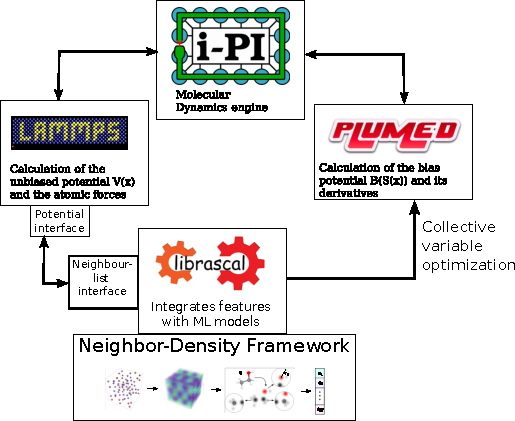
\includegraphics[width=\textwidth]{fig/ipi-librascal-plumed.pdf}
    \caption{A schematic showing the interwork of the software packages to run metadynamic simulations to study paraelectric-ferroelectric phase transitions in barium titanate. The domain decomposition of \texttt{LAMMPS} is noted as $\mathbf{q}$ for the full atomic position vectors and $[\mathbf{q}^{(1)},\ldots, \mathbf{q}^{(C)}]$ for the positions corresponding to the $C$ domains.} 
    \label{fig:ipi-librascal-plumed}
\end{figure}

\subsection{Finite-size convergence of the Curie point in barium titanate}

\begin{figure}
    \centering
    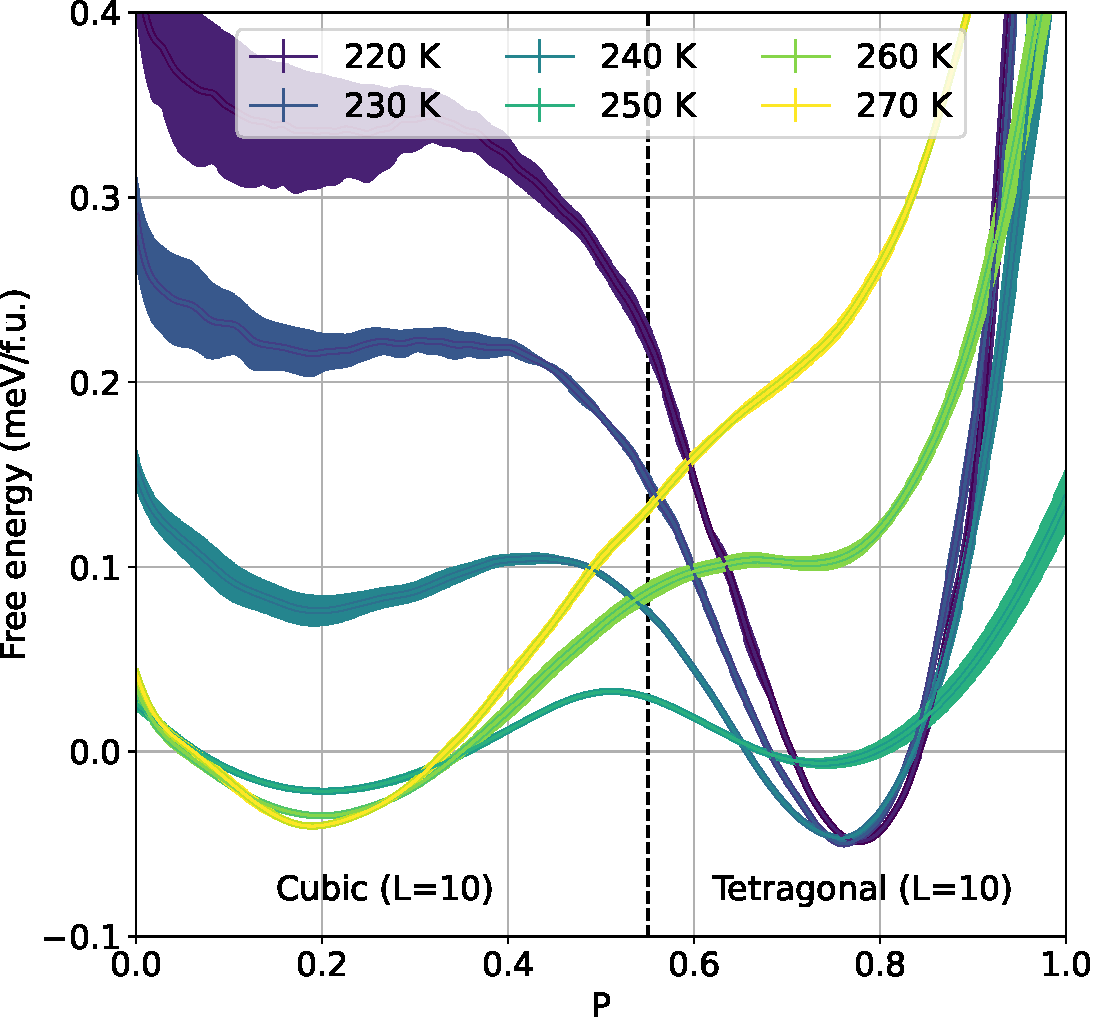
\includegraphics[width=0.7\linewidth]{fig/Free-energy_vs_P_101010.pdf}
    \caption{Free energy surfaces as a function of the collective variable for temperatures above and below the transition temperature (249 K) for a $10\times10\times10$ cell. The shaded areas correspond to errors on the free energy, computed as the standard deviation on the mean of the free energy estimates on 4 independent blocks for each metadynamics simulation.}
    \label{fig:1D-free-energy}
\end{figure}

\begin{figure}
    \centering
    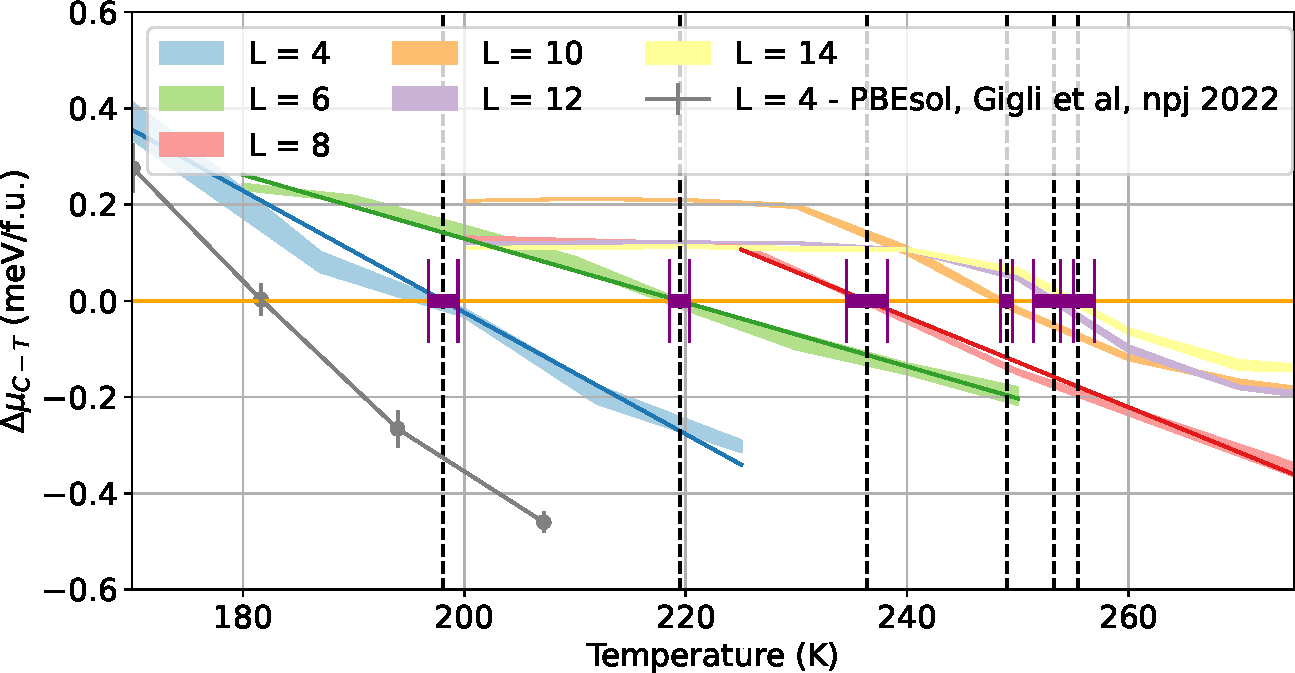
\includegraphics[width=0.8\linewidth]{fig/Size-scaling-deltamu.pdf}
    \caption{Difference between the chemical potential of the cubic and tetragonal phases as a function of the temperature for different simulation box sizes $L$.}
    \label{fig:size-scaling-delta-mu}
\end{figure}

In previous work~\cite{gigli_thermodynamics_2022} a transition between the cubic and tetragonal phases was observed in unbiased MD simulations of $4\times4\times4$ supercells.  These transitions occur in unbiased MD because the cell is relatively small.  When a larger supercell is employed spontaneous transitions become exceedingly rare and the system remains stuck in the energetic minimum that corresponds to the cubic or tetragonal phase for the duration of the simulation.  For these larger systems a simulation bias is thus required to drive transitions between the two phases.  Fig.~\ref{fig:1D-free-energy} shows that metadynamics simulations using the order parameter based on the Ti-centered spherical expansion coeffients in the notation as in Eq.~\eqref{eq:chemical_decomposition}
\begin{equation}
  P = \sqrt{(\sum_{i\in A} c_{O11-1}^i)^2 + (\sum_{i\in A} c_{O110}^i)^2 + (\sum_{i\in A} c_{O11+1}^i)^2}, 
\end{equation}
can be used to drive  transitions for $10\times10\times10$ supercells. This figure shows the free energy surfaces (FES) that emerge from these metadynamics simulations. These free energy surfaces were obtained by reweighting using the iterative trajectory reweighting (ITRE) method \cite{giberti_iterative_2020}.  Block averaging was used to estimate the errors on the estimates of the free energy shown in figure \ref{fig:1D-free-energy}. 

Fig.~\ref{fig:1D-free-energy} clearly shows that there is a minimum for high CV values when the temperature is low and the system is in the tetragonal phase and ferroelectric. This minimum is replaced by a minimum at a low value of the CV when the temperature is high and the system is in the cubic phase and paraelectric.  At intermediate temperatures two minima are observed as one phase is metastable.

To extract the difference in chemical potential between the tetragonal and cubic phases we performed clustering using the probabilistic analysis of molecular motifs algorithm (PAMM) \cite{gasp+18jctc}. This clustering technique assigns two probabilities $\theta_1(s_i)$ and $\theta_2(s_i)$ to each CV value $s_i$.  $\theta_1(s_i)$ is the likelihood that the corresponding frame is from the cubic basin, while  $\theta_2(s_i)$ measures the likelihood that it is from is tetragonal basin. The chemical potential difference per formula unit between the two phases can thus be estimated as:
$$
\Delta\mu_{\textrm{C-T}} = -\frac{k_B T}{L^3} \log \left( \frac{\sum_i \theta_1(s_i) w_i}{\sum_i \theta_2(s_i) w_i} \right) 
$$
where the sum runs over all the trajectory frames, $L^3$ is the number of unit cells, $T$ is the temperature and $w_i$ is the weight for each trajectory frame obtained from ITRE.  

\begin{figure}
    \centering
    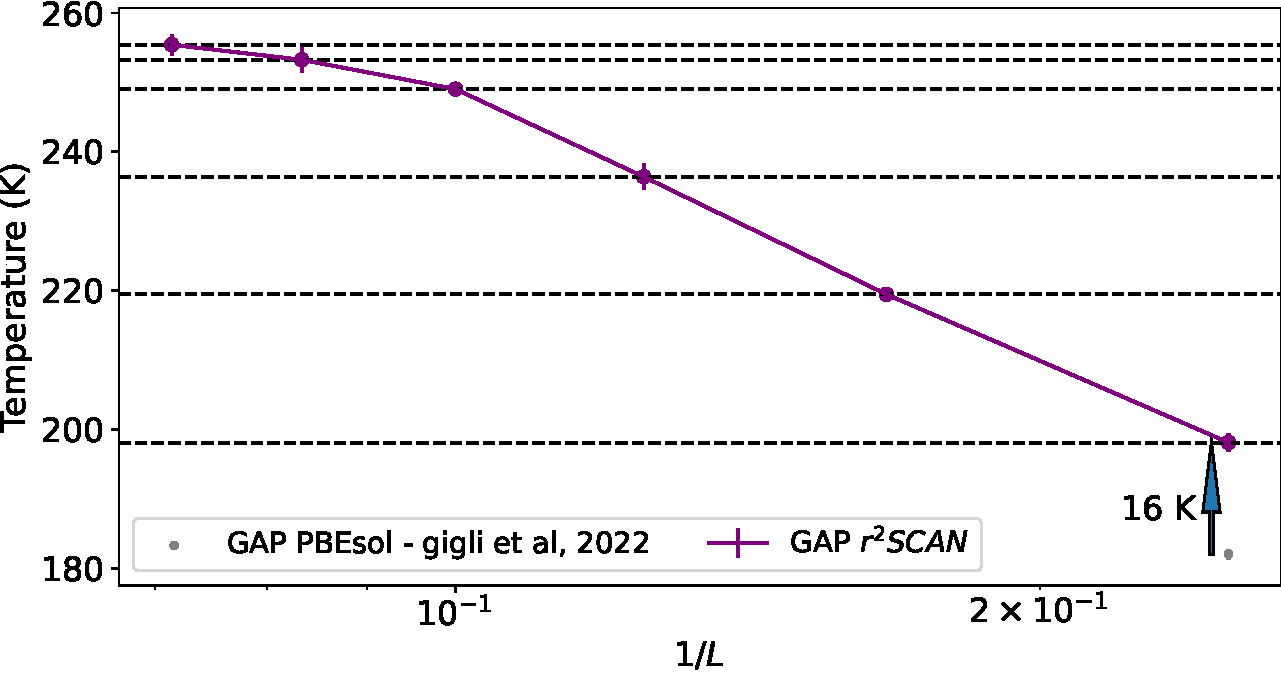
\includegraphics[width=0.8\linewidth]{fig/Size-scaling-Temp.pdf}
    \caption{Predicted Curie point at a function of the inverse of the box size $1/L$.  The grey dot at the bottom right shows the result from \cite{gigli_thermodynamics_2022}. The more accurate functional used in this work shifts the transition temperature upwards by 16 K as indicated by the vertical arrow. However, this upward shift is smaller than the increases in transition temperature that are seen for the larger systems simulated in this work.}
    \label{fig:size-scaling-temp}
\end{figure}

Fig.~\ref{fig:size-scaling-delta-mu} shows how $\Delta\mu_{\textrm{C-T}}$ changes with temperature for a range of differently-sized supercells.  This quantity is initially positive for all cell sizes indicating that the tetragonal phase is more stable than the cubic one at low temperatures.  It becomes negative at high temperatures when the relative stabilities of the two phases reverses.  The Curie point can be determined from figure  \ref{fig:size-scaling-delta-mu} by finding the temperature at which $\Delta\mu_{\textrm{C-T}}$ is zero.  In figure \ref{fig:size-scaling-delta-mu} these temperatures are indicated by the vertical dashed lines.  Errors on these estimates of the Curie temperature are also indicated. To determine these errors we divided each trajectory into four blocks and obtain four separate estimates for each $\Delta\mu_{\textrm{C-T}}$ value.  Variances were computed from these four estimates so the shaded areas in figure \ref{fig:size-scaling-delta-mu} indicate the (1-$\sigma$) confidence limits.  The Curie temperature for each system size was extracted by drawing a line of best fit through the estimates of    $\Delta\mu_{\textrm{C-T}}$.  Propagated errors from this fitting then yield an estimate of the error on the transition temperature.

Figure \ref{fig:size-scaling-delta-mu} clearly shows that the Curie temperature increases with system size.  Furthermore, these differences in transition temperature are for the most part statistically significant.  Figure \ref{fig:size-scaling-temp} indicates the size dependence for the transition temperature more clearly.  In this figure the transition temperature is shown as a function of the inverse box size.  It is only the $14\times14\times14$ system that has a transition temperature that is compatible with the smaller  $12\times12\times12$ system.  For all other system sizes the transition temperature is  underestimated. The observation of significant finite-size effects here contradicts the analysis provided in Ref. \cite{gigli_thermodynamics_2022} that relied on extrapolating the dielectric constant in the high-temperature regime with a Curie-Weiss law. Interestingly, this indirect approach underestimates the finite size effects. If the aim is to extract accurate thermodynamics simulating large system sizes is thus essential.




%In this framework \texttt{LAMMPS} is only used for the MPI parallelization of the neighborlist as the dynamics are managed by \texttt{i-PI} and the energy and force calculation by \texttt{librascal}.
%---
%\begin{subequations}
%\begin{align}
%  \tilde{P}(s) &\propto \int\mathrm{d}\mathbf{q}\,\exp(-\frac{\tilde{V}(\mathbf{q})}{T})\delta(\mathbf{s}-S(\mathbf{q})\\
%  F(\mathbf{q}) &= -\int\mathrm{d}\mathbf{q}^\prime V(\mathbf{q}^\prime)\delta(\mathbf{q}^\prime -\mathbf{q}) + C
%\end{align}
%\end{subequations}
%developed \texttt{i-PI}.
%integrate the develo
%As a full recovery of the free energy surface is infeasbile for any realistic system due to the dimensionality of the configuration space $\mathbf{q}\in\mathbb{R}^{3N}$, it is common method to act on a reduced collective variable space $\mathbf{s}\in\mathbb{R}^d$.
%
%\begin{equation}
%  F(\mathbf{q}) = -T\log(P(\mathbf{q})),
%\end{equation}
%Then to accelerate the sampling rate of the is to perform metadynamics~\cite{}.
%to accelerate the sampling of the transition.
%It adds a bias potential to the potential $B$ that acts on a reduced collective variable space $\mathbf{s}\in\mathbb{R}^d$, 
%\begin{equation}
%  \tilde{V}(\mathbf{q}) = V(\mathbf{q}) + B(S(\mathbf{q})), S:\mathbb{R}^{3N}\rightarrow\mathbb{R}^d,
%\end{equation}
%where $S$ is a function that retrieves the collective variable from the configuration.
%By sampling from the canonical distribution associated with the potential
%\begin{subequations}
%\begin{align}
%  \tilde{P}(s) &\propto \int\mathrm{d}\mathbf{q}\,\, \exp(-\frac{\tilde{V}(\mathbf{q})}{T})\delta(\mathbf{s}-S(\mathbf{q})\\
%               &= \exp()\\
%  F(\mathbf{q}) &= -\int\mathrm{d}\mathbf{q}^\prime V(\mathbf{q}^\prime)\delta(\mathbf{q}^\prime -\mathbf{q}) + C
%\end{align}
%\end{subequations}
%One can retrieve the free energy
%\begin{equation}
%  \log(\tilde{P}(s)) \int\mathrm{d}\mathbf{q}\,\, \exp(-\frac{\tilde{V}(\mathbf{q})}{T})\delta(\mathbf{s}-S(\mathbf{q}))
%\end{equation}
%Typically $\mathbb{R}^d$ is limited up to three dimensions due to computational complexity.
%that is later normalized out in the calculation of the free energy.
%While the forces of the MLIP were computed with \texttt{LAMMPS} and the forces of the bias potential were computed with \texttt{PLUMED}\cite{PLUMED}.
%To consolidate both forces for the metadynamics the software-package \texttt{i-PI} was used, that implemented a custom protocol to each of these MD packages to allow communicatiof the forces to a python interface.
%A schematic of the interwork between the software packages can be seen in Fig.~\ref{fig:ipi-librascal-plumed}.
%\begin{figure}
%    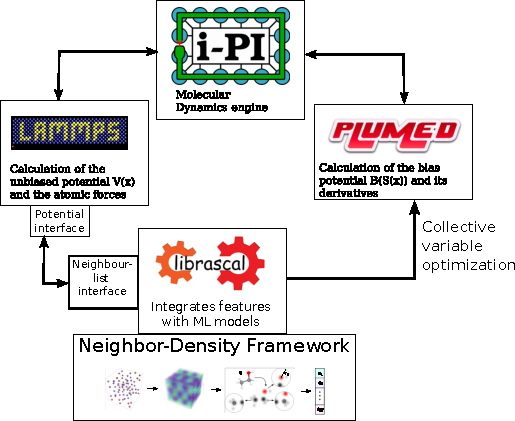
\includegraphics[width=\textwidth]{fig/ipi-librascal-plumed.pdf}
%    \caption{A schematic showing the interwork of the software pieces to run metadynamic simulations to study interfacial effects of barium titanate.}
%    \label{fig:ipi-librascal-plumed}
%\end{figure}
%
%As CV for the metadynamics $l=1$ components of the spherical expansion coefficients computed with \texttt{librascal} were used.
%My implementation of the cubic spline helped to speed up the computation of the bias term.
%Since only the expansion coefficients centered for the oxygen neighbors centered on the titanate was sufficient for the CV, I further implemented an option to selectively computate the partial gradients for certain species.
%Note that a selectional computation of partial gradients also needs to consider dependencies of the gradient on the central energies of its neighbors as pointed out in Eq.~\eqref{eq:forces_interatomic_potential}.
%implementation of was implemented by me to speed up the metadynamics simulation
%work are adjustments to the
%In the subsequent sections we will discuss the technica
%My contributions to this work was firstly, to participate in the development of the MLIP package \texttt{librascal} that was used to conduct DFT simulations at higher levels-of-theory to analyse its effect on the temperature.
%Specifically, the implementation of selective computations of the partial gradients for certain species was implemented by me to speed up the metadynamics simulation.
%Secondly, the implementation of an interface to the MD software \texttt{LAMMPS} that allowed to study the finite size effects on the Curie temperature.

%The interface was implemented by Gareth Tribello.

%\section{Modular design of MLIP}
%As scientific methods continue to evolve, the demands placed on software to incorporate these advancements also grow.
%%While advances in methodolgy can prove to improve a method in all aspects, and thus replace an existing method, it is more often the case that they extend the capabilities and requiring more flexibility of the software outside of the initial design of the software package.
%While improvements in method development often lead to enhanced efficiency and user-friendliness, they typically extend the software's capabilities beyond its original design.
%As software is extended by more features over time, it tends to become less adaptable to changes to incorperate newly developed methods.
%Consequently, rapid advancements in methodology can render software obsolete before the development is even at the stage of deployment for experiments.
%%Considering that software becomes more rigid to changes over time with increased number of implemented features, it is a natural consequence that with a rapid development in methodology the software becomes deprecated as it cannot keep up with these changes.
%Similar challenges were observed in the 1960s when rapid hardware development contributed to a software crisis\cite{brian2012software_crisis}.
%However, as development progresses, also the understanding of critical components for performance emerges which solidifies the possible software designs to retrieve performant code.
%With this places in the software naturally appear that can be used to decompose it into separate components allowing to distribute the software development workload among peers.
%%groups as they can independently work on the individual modules.
%This not only allows to speed up the development but it also allows a more specialized development leading to more performant code.
%While scientific publications cover abundantly method development based on mathematical advancements, the modular design of software implementing a variety of methods in a specific domain is still highly underrepresented in the scientific literature even though it dictates the efficiency the method development.
%%With regard to incensitives present academia that only fund software development tied to new scientific applications, the existing fragmented landscape of unmaintained monolothic software packages solving over and over again the same problem is a natural consequence.
%%Advances can be only made when enough money is allocated to a group that recognizes the need to create a software package standardizing interfaces.
%This section discusses modular design patterns relevant for the domain of atomistic learning to integrate of machine learning interatomic potentials with molecular dynamics packages.
%Interfaces where applicable are needed to reduce software costs for groups focusing on optimization of .
%Modular design is essential for sustainable scientific problem: Not reinventing the wheel, extensibility, wider-applicability, focused problem-solving
%The production of reliable and maintained software is essential for the progress of further scientific development to  prevent a scientfic crisis as in the \cite{TODO}.
%
%%\section{MLIP}
%%A common approach for the integration of machine learning into the molecular dynamics simulation
%%\begin{equation}
%%  H(\mathbf{p}, \mathbf{q}) = \frac{\mathbf{p}^2}{2m} + V(\mathbf{q})% + theromstat/barostat
%%\end{equation}

%Note that contributions to the gradient come from the partial gradients $\partial E_k/\mathbf{r}_{jk}$ 
%wrt. to the distance vector to all neighbors 
%\emph{and} from $\partial E_j/\mathbf{r}_{kj}$ where $j$ is in the neighborhood of atom $k$ ($j\in A_k$). 
%additional pr to be done to allow contiguous iteration during the computation of the gradients.

%Note that one can simplify the gradients for further usage by summing neighbour and central contributions
%\begin{subequations}
%\begin{align}
%  \mathbf{F}_{kj} = -\frac{\partial E_k}{\mathbf{r}_{jk}} + \frac{\partial E_j}{\mathbf{r}_{kj}} \\
%  \frac{\partial E_A}{\partial\mathbf{r}_k} = \sum_{j\in A_k} \mathbf{F}_{kj}.
%\end{align}
%\end{subequations}

%\cite{https://docs.lammps.org/Developer_write_pair.html}
%As classical molecular dynamics simulation require the computation

%In this section we will discuss the approach that is taken in software for classical molecular dynamics code as \cite{LAMMPS, Gromacs, CP2K, Plumed, Jaxmd, OpenMMTODO}.
%%equilibrium hat uses the Born-Oppenheimer approximation 
%%software simulating equilibrium dynamics using the Born-Oppenheimer approximation so 
%%equilibrium hat uses the Born-Oppenheimer approximation 
%%A common approach for equilibrium molecular dynamics software is to 
%From the equations of motion 
%\begin{subequations}
%\begin{align}
%  H(\mathbf{p}, \mathbf{q}) = \frac{\mathbf{p}^2}{2m} + V(\mathbf{q}),\\% + theromstat/barostat
%  \frac{\partial\mathbf{p}}{\partial t} = \frac{\partial V(\mathbf{q})}{\partial\mathbf{q}}, \\
%  \frac{\partial\mathbf{q}}{\partial t} = \frac{\partial \mathbf{p}}{m},
%\end{align}
%\end{subequation}
%we obtain 
%a separation of the computation of kinetic and potential energy into separated modules arises.
%Depending on the type of thermodynamic ensemble and subsequently the thermo- or barostat the kinetic energy and its derivative, the differently evaluated.
% TODO I don't know if these are really easy changes
%As the evaluation of the kinetic energy, even considering the correction by thermo- or barostat, is computationally not significant, a lot of method development and specialized software has been focused on making the evaluation of the potenial energy more efficient.

%The potential energy can be further separated into a short- and long-range term
%\begin{equation}
%  V(\mathbf{q}) = V_\textrm{short}(\mathbf{q}) + V_\textrm{long}(\mathbf{q}).
%\end{equation}
%Often MD software separate the calculation of both parts into separate module as $V_\textrm{short}$ is computed in real space and the $V_\textrm{long}(\mathbf{q})$ typically is computed in Fourier space as much is not reused thus not much can be recomputed.
%Therefore both require different types of data structures  and resolved in complicated 
%and therefore the separation into separate modules naturally arises.
%
%take computationally advantage of using a neighborlist using binning (also known as voxel) algorithms\cite{TODO} while the long-range part can be computationally efficient evaluated in Fourier space using partical mesh methods\cite{TODO}.
%Under the assumption of uniformly distributed system the theoretical complexity is $O(N\log N)$ instead of $O(N^2)$ in the implementation of naive scaling.
%Even though a perfect uniform distribution is almost never fulfilled for a system, it is reasonable to assume one is close enough to such a state for a large part of the states during a simulation that the theoretical scaling is approximative true.
%Note that theoretical scaling arguments completely ignore constant overheads due to preprocessing or improvements due to hardware capacities (e.g. cache locallity, hardware capability of parallel processing) that are essential for real applications. 

%MPI pair contributions of forces requiring reorganisation of contributions to consider ghost neighbors correctly.
%One advantage for such a separation is that the implementation of the thermo- and barostats different ensembles, the calculation of the neighborlist can be separated in different parts of the code.
%optimization of the calculation of the neighborlist can be separately
%An advantage of the development of software dedicated for the creation of interatomic potentials separate from the other parts of the MD software.
%The parts that control how the MD work thus do not need be reimplemented and optimizations of the neighborlist with MPI can be reused.
%A disadvantage of the modularity can be seen in example for a long-range potential.
%While usually 

%\subsection{Application LAMMPS Plumed interface for interfacial effects on BaTiO3}

%\section{Modularity in MLIP}
%There are several things we learn from technical analysis details that prevent a modular design as present it exists for traditional machine learning algorithms.
%Narative:
%An essential prevention for modularity is that the computation of the kernel requires a sparse data format hash mappable due to the species polynomial growth
%Secondly, most ML packages do not support gradients in their methodology.
%A recent develompent.

%\subsection{MLIP interface}

\section{Future work}
The development on \texttt{librascal} has revealed several disadvantages in the design that required to rethink the general approach of creating an ecosystem for the construction of MLIP.
This redesign can be attributed to the lack of modularity and serialization of models that are discussed in the following in more detail. 

\subsection{Modularity of featurization and model construction}
A crucial disadvantage in the design of \texttt{librascal} was the entanglement of the featurization and the model construction inside one library.
This entanglement is required to efficiently compute the forces as indicated in Eq.~\eqref{eq:efficient_kernel_evaluation}, since it does not allow a separate computation of the weights and kernel derivatives.
% that is required for utilizing packages as \texttt{scikit-learn} for the model computation.
To implement Eq.~\eqref{eq:efficient_kernel_evaluation} it requires a common data format for the features and model to operate.
%Tth the specific mean of ecah
This requires to include the indices of each dimension of the features and its gradients into a well-defined data format, such as the atomic species, local environment and structures.
%the model ne, requires an understanding of the decomposition of the target property into local contributions Eq.~\eqref{eq:structural_separation} as well as an understanding of the relationship between features and gradients.
That problem is tackled by the development of a new software package \texttt{metatensor}.
The package offers a data structure that acts as a container of the feature and its gradients by storing the labels the individual dimensions.
This allows \texttt{numpy}-like data manipulation that takes structural characteristics of the data into account.
With that kind of data structure the model and featurization can be separated into two different packages, since the relevant structural information of the features and gradients is kept in the data output.
That effort is currently in progress with the development of \texttt{rascaline} and \texttt{torch\_spex}, packages for the featurization of atomic structures returning them as \texttt{metatensor} data containers, and \texttt{metatensor-learn} a subpackage for the model construction from \texttt{metatensor} data containers.
%he feature and their attribution to these structural characteristics as well to its gradients


%For that software package \texttt{metatensor} allows to attribute these structural characteristics to the object itself as metadata and offers \texttt{numpy}-like data manipulations that take advantage of the metadata.
%This allowed a disentanglement of the featurization that has reimplemented in a new package \texttt{rascaline} and model construction that has been moved to \texttt{equisolve}.
%Part of my contribution was to participate in the development of \texttt{metatensor} as well as heavily developing on the initial design of \texttt{equisolve} contributing module of shallow methods including standardizer, linear and the above-presented kernel model as well as the inital designs for neural network models based on the data formate created in \texttt{metatensor}.
%
%While the term $\partial\mathbf{c}_i/\partial\mathbf{r}_k$ depends solely on the choice of featurization, the term $\partial k_t(\mathbf{c}_i)/\partial\mathbf{c}_i$ depends on the choice of kernel, thus the computation of the kernels and featurizations can be separated.
%A problem that arised in \texttt{librascal} is that the species introduce a high structural sparsity in the features that needs to be also considered in the kernel computation to be efficient.
%For that the kernel needs to support understand the structural sparsity pattern and could remain agonstic to the form of featurization.
%While there exist multiple sparsity formats\cite{}, they are agnostic to the structure of the data and thus do not allow us to exploit structural sparsities that depend on specif information as the species.
%Furthermore as we saw in the last sections, to predict gradients with kernel a high dependency with the featurization arises that do not allow existing domain agonistic approaches as in packages as \texttt{sckitit-learn}.
%To solve this problem a new data-container package, named \texttt{metatensor}, has been designed that supports structural sparsity by assigning metainformation to the dimensions of tensors and stores features and their gradients within the same data object such that consistent manipulation of the features and gradients can be done.
%With this direction a disentanglement of the existing model is possible, allowing a much more modular approach.
%managers
\subsection{Serialization of MLIPs}
ML models exhibit various trade-offs between accuracy, evaluation time, training cost, and hyperparameter optimization.
Consequently, the choice of a suitable model depends on the system of interest, the size of the dataset, and the available computational resources.
%A significant challenge arises from the current software infrastructure supporting ML models for MD software.
%The current software infrastructure of ML models for MD software causes a lot of friction when the model type is changed, as 
In the last decade, the rapid development of machine learning models has produced numerous interfaces for MD engines such as \texttt{LAMMPS}~\cite{lammpsmliap,lammpsmlpace,lammpsmlpod,lammpsmlquip,lammpsmlhdnnp}.
The current software infrastructure, however, causes considerable friction between the ML package and the MD code when switching the model.
In fact not only the MD software requires a recompilation for a different interface and an installation of  a new package but also a whole new workflow for training and deployment needs to be often created.
In addition, the model development frequently takes place in higher-level languages like \texttt{Python} or \texttt{Julia}, owing to their flexibility.
The choice of the programming language for model development narrows down its deployment to MD packages that provide compatible interfaces for that exact language, otherwise the they require an implementation of the model in one of the supported languages that the MD engine provides.
This requires an additional implementation of a process that saves the model to a file that can be loaded back from the low-level language interface.
The process of exporting a data structure to file is named \emph{serialization}.
This additional development work hinders the application of numerous developed ML models in MD packages written low-level programming languages, which are essential for researching large systems or conducting long-term simulations.


Similar challenges are present in the industry, where models trained with diverse ML packages must be adapted to various hardware architectures and software stacks.
This diversity complicates the consistent deployment of the same package version across different devices.
To address this, an open intermediate representation for ML models, known as \emph{open neural network exchange} (ONNX), has been developed ~\cite{bai2019}.
However, ONNX is currently not a suitable candidate to serialize MLIPs, since it does not support the inference of gradients.

The \emph{open knowledgebase of interatomic models} (OpenKIM) ~\cite{karls2020openkim} attempts to solve this issue by developing abstract representations of data and processing directives necessary for molecular simulations.
It unifies several MD packages to one common molecular dynamics to interatomic potential interface, named the KIM API~\cite{elliott2011kim}.
Although this approach reduces the number of required interfaces, it doesn't comprehensively cover all relevant MD packages.
Notably, packages like \texttt{GROMACS} and \texttt{CP2K}~\cite{kuhne2020cp2k} are absent.
Most MD packages supported by the KIM API are implemented in higher-level languages, which in the first place do not present a hurdle for MLIP developers to interface with.
However, this solution does not allow a full development of MLIPs in a high-level language, as it still necessitates the creation of an interface with the KIM API using a low-level language such as C, C++, or Fortran.

It is due to the shortcoming of the existing solutions that we pursue a software ecosystem that leverages TorchScript as serialization format.
TorchScript not only supports the inference of gradients but allows a model utilization in C++, overcoming the high-level to low-level language barrier.
Additionally, it offers advanced model optimization utilities, such as kernel fusioning, to enhance complex models' efficiency.
Considering these capabilities, TorchScript appears to be a promising candidate to standardize the landscape of MLIPs.

%They developed abstract representations of the data and processing directives necessary to perform a molecular simulation thereby unifying the interfaces of several MD packages to one interface, namely the KIM API.
%While it reduces the cost of the number interfaces that are needed, they are far from covering comprehensively all relevant MD packages, as packages like GROMACS~\cite{hess+08jctc} and C2PK~\cite{kuhne2020cp2k} are missing.
%Most of the supported MD packages are implemented in higher-level languages for which a custom MLIP interface can be easily implemented.
%
%A solution we target with the software ecosystem developed in our lab is to use TorchScript as it supports the use of gradients and offers a usage of the model in C++ surpassing the high-level language barrier.
%It further supports advances model optimization utilities that can be used optimize complex models by kernel fusioning of the operation graph.
%Considering all that it seems like a promising candidate to standardize the landscape of MLIPs.




%In last decade, the rapid development of machine learning models has resulted in numerous interfaces for \texttt{LAMMPS}\cite{QUIP}. %TODO more
%%While the model accuracy is a good indicator for the usability of a model, it is still not reliable enough to be a guarantee that the model will work for MD software as undersampling of the phase space can always be an issue for any kind of model.
%%One is therefore forced to retrain the model for a dataset covering a larger part of the phase pace or switch to a more accurate model during the analysis of an experiment.
%As ML models show different trade-offs between accuracy, evaluation time, trainings cost and hyperparameter optimization the set of suitable models depend on the system of interest, the dataset size and the given computational resources.
%%As the dataset size changes over the course of analysis different models become more suitable candidates and thus a different model is more suitable for the analysis.
%%It has been shown that linear models can be competetive in high data regime. %TODO verify that
%The current software infrastructure of ML models for MD software causes a lot of friction when changing the model type as the MD software needs to be recompiled for a different interface. % and a new workflow pipeline has to be constructed.
%Even more crucial is the fact that the model development is often conducted in higher-level languages like \texttt{Python} or \texttt{Julia} due to their flexibility.
%This however restricts the deployment of the model to MD packages that offer a potential interface in the same language as the model supports.
%%implementation of a serialization for the model plus interface for an MD package.
%This restricts the deployment of numerous developed ML models in low-level MD packages which are often required to conduct research on large systems or for long time-scales.
%%For nearly five years following its initial publication, the widely-used SchNet model\cite{schu+18jcp} lacked an interface with a low-level MD package.
%%This however restricts the usage of the model also to higher-level when no serialization exists. 
%%Heteregoneous hardware optimizer: OneAPI, Kokkos
%
%Similar problems exists in industry where models trained with different ML packages need to be shipped to devices with different hardware architectures and different software stacks making it hard to reliably provide the same version of the package on each device.
%In industry therefore an open intermediate representation for machine learning models has been developed named \emph{open neural network exchange} (ONNX).
%This standard can however not be used for MLIPs as they lack the support of the inference for gradients.
%%Since the majority of ML models are constructed in higher-level languages, most MD engines are written in a low-level language for performance reasons.
%%It is thus needed to export models to a standardized formate that allows to execute models in the low-level languaes
%%Low-level language for efficiency, scripting-like for flexibility
%
%%to export models to one software from memory to disk for reproducibility and hardware independency (e.g. JSON).
%
%The Open Knowledgebase of Interatomic Models (OpenKIM)\cite{karls2020openkim} tries to address the problem.
%They developed abstract representations of the data and processing directives necessary to perform a molecular simulation thereby unifying the interfaces of several MD packages to one interface, namely the KIM API\cite{elliott2011kim}.
%While it reduces the cost of the number interfaces that are needed, they are far from covering comprehensively all relevant MD packages, as packages like GROMACS\cite{hess+08jctc} and C2PK\cite{kuhne2020cp2k} are missing.
%Most of the supported MD packages are implemented in higher-level languages for which a custom MLIP interface can be easily implemented.
%
%A solution we target with the software ecosystem developed in our lab is to use TorchScript as it supports the use of gradients and offers a usage of the model in C++ surpassing the high-level language barrier.
%It further supports advances model optimization utilities that can be used optimize complex models by kernel fusioning of the operation graph.
%Considering all that it seems like a promising candidate to standardize the landscape of MLIPs.

%\section{Foreign-Function interface [optional]}
%Low-level language for efficiency, scripting-like for flexibility
%Libraries that https://www.swig.org/compat.html
%Check out \url{https://docs.rs/rust_swig/latest/rust_swig/#enums}
%However these are not working with TorchScript, also Julia is missing that is becoming essential for scientific softwared development

%\section{Machine learning ecosystems}
%
%\subsection{Hardware kernels}
%\subsection{scikit-learn - close-form inspired infrastructure}
%- transformers, models
%- fit function needs to be specified that optimizes one object
%- concatenation of models through Pipelines allows parameter optimization over different modules however it is every rigid (sample dimension cannot change over the pipelines)
%\subsection{torch - autograd inspired infrastructure}
%Dataloader:
%- concatenation of indicies
%- caching
%Optimizer:
%- concatenation of indicies
%- caching
%While torch summarizes all existing optimizers under one library, Jax approaches this issue with modularity\cite{jaxopt_implicit_diff}
%\subsection{Standardization array-APIs}
%mention Array-API
%https://data-apis.org/array-api/latest/

%\section{MLIP for applications on ferroelectrics}
%\section{Metadynamic framework using MLIP}
%We have seen development of splining algorithms.
%In the chapter we cover a specific application where this supported the work
%
%A ferroelectric is a material that possesses a permanent electric polarization that can be switched under the action of an external electric field.
%Typically, the emergence of the polar phase is accompanied by a structural transition from a high-symmetry paraelectric state down to a broken-symmetry state with a characteristic long-range dipolar ordering [1, 2].
%Early studies on ferroelectrics using ab-initio calcluation [23, 24] have identified discrepancies between the temperatures at which structural transitions occur in the simulations and the temperatures at which these transitions occur in reality.
%These discrepancies are often reduced by introducing artificial corrections to the simulated pressure [25–27].
%This additional pressure brings the simulation volume closer to the values seen in experiments and drives the predicted Curie temperature towards its experimental value.
%However, this correction tells us little about the physical origins for the discrepancies that are observed in simulations.
%There are multiple sources of error that could be the origin for these discrepancies.
%(1) The GGA functional (PBEsol) [28] used in previous work slightly underestimates the equilibrium volume of cubic BaTiO3.
%(2) The determination of the transition temperature by tracking spontaneous fluctuations between the phases limits the system size that can be studied, despite the reduced computational cost of the ML potential.
%The paraelectric-ferroelectric phase transition needs to be therefore studied by using metadynamics simulations.
%
%%work are adjustments to the
%%In the subsequent sections we will discuss the technica
%%My contributions to this work was firstly, to participate in the development of the MLIP package \texttt{librascal} that was used to conduct DFT simulations at higher levels-of-theory to analyse its effect on the temperature.
%%Specifically, the implementation of selective computations of the partial gradients for certain species was implemented by me to speed up the metadynamics simulation.
%%Secondly, the implementation of an interface to the MD software \texttt{LAMMPS} that allowed to study the finite size effects on the Curie temperature.
%
%To conduct metadynamics a bias term based on the spherical expansion coefficients was computed \texttt{PLUMED} using \texttt{librascal}
%%The interface was implemented by Gareth Tribello.
%To consolidate the forces computed with \texttt{LAMMPS} and the bias term computed with \texttt{PLUMED} to run metadynamics the software-package \texttt{i-PI} was used, that implemented a custom protocol to each of these packages to allow communication betwe.
%A schematic of the interwork between the software packages can be seen in Fig.~\ref{fig:ipi-librascal-plumed}.
